\documentclass[a5paper, 10pt]{article}

% Текст
\usepackage[utf8]{inputenc} % UTF-8 кодировка
\usepackage[russian]{babel} % Русский язык
\usepackage{indentfirst} % красная строка в первом параграфе в главе
% Отображение страниц
\usepackage{geometry} % размеры листа и отступов
\usepackage{listings}
\usepackage{color}

\usepackage{float}
\floatplacement{figure}{H}

\geometry{
	left=12mm,
	top=25mm,
	right=15mm,
	bottom=17mm,
	marginparsep=0mm,
	marginparwidth=0mm,
	headheight=10mm,
	headsep=7mm,
	nofoot}
\usepackage{afterpage,fancyhdr} % настройка колонтитулов
\pagestyle{fancy}
\fancypagestyle{style}{ % создание нового стиля style
	\fancyhf{} % очистка колонтитулов
	\fancyhead[LO, RE]{ЛР № 5 } % название документа наверху
	\fancyhead[RO, LE]{Типовые динамические звенья} % название section наверху
	\fancyfoot[RO, LE]{\thepage} % номер страницы справа внизу на нечетных и слева внизу на четных
	\renewcommand{\headrulewidth}{0.25pt} % толщина линии сверху
	\renewcommand{\footrulewidth}{0pt} % толцина линии снизу
}
\fancypagestyle{plain}{ % создание нового стиля plain -- полностью пустого
	\fancyhf{}
	\renewcommand{\headrulewidth}{0pt}
}
\fancypagestyle{title}{ % создание нового стиля title -- для титульной страницы
	\fancyhf{}
	\fancyhead[C]{{\footnotesize
			Министерство образования и науки Российской Федерации\\
			Федеральное государственное автономное образовательное учреждение высшего образования
	}}
	\fancyfoot[C]{{\large 
			Санкт-Петербург, 2025
	}}
	\renewcommand{\headrulewidth}{0pt}
}

%Программирование
\usepackage{listings}

\definecolor{codegreen}{rgb}{0,0.6,0}
\definecolor{codegray}{rgb}{0.5,0.5,0.5}
\definecolor{codepurple}{rgb}{0.58,0,0.82}
\definecolor{backcolour}{rgb}{0.95,0.95,0.92}

\lstdefinestyle{codestyle}{
    backgroundcolor=\color{backcolour},
    keywordstyle=\color{magenta},
    numberstyle=\tiny\color{codegray},
    stringstyle=\color{codepurple},
    basicstyle=\ttfamily\footnotesize,
    breakatwhitespace=false,
    breaklines=true,
    captionpos=b,
    keepspaces=true,
    numbers=left,
    numbersep=5pt,
    showspaces=false,
    showstringspaces=false, % показывать или нет пробелы специальными отступами
    showtabs=false, % показывать или нет табуляцию в строках
    tabsize=2 % размер табуляции по умолчанию равен 2 пробелам
}
\lstset{
    language=Python, % Язык программирования
    basicstyle=\ttfamily\small, % Стиль текста
    commentstyle=\color{green}, % Стиль комментариев
    keywordstyle=\color{blue}, % Стиль ключевых слов
    stringstyle=\color{red}, % Стиль строк
    showstringspaces=false, % Не показывать пробелы в строках
    breaklines=true, % Переносить длинные строки
    extendedchars=true, % Поддержка кириллицы
    inputencoding=utf8, % Кодировка входного файла
    numbers=left,               % где поставить нумерацию строк (слева\справа)
    numberstyle=\tiny,           % размер шрифта для номеров строк
    stepnumber=1,                   % размер шага между двумя номерами строк
    numbersep=5pt,                % как далеко отстоят номера строк от подсвечиваемого кода
    captionpos=b,              % позиция заголовка вверху [t] или внизу [b] 
    breaklines=true,           % автоматически переносить строки (да\нет)
    breakatwhitespace=false, % переносить строки только если есть пробел
    literate={а}{{\cyra}}1 {б}{{\cyrb}}1 {в}{{\cyrv}}1 {г}{{\cyrg}}1 {д}{{\cyrd}}1
             {е}{{\cyre}}1 {ё}{{\cyryo}}1 {ж}{{\cyrzh}}1 {з}{{\cyrz}}1 {и}{{\cyri}}1
             {й}{{\cyrishrt}}1 {к}{{\cyrk}}1 {л}{{\cyrl}}1 {м}{{\cyrm}}1 {н}{{\cyrn}}1
             {о}{{\cyro}}1 {п}{{\cyrp}}1 {р}{{\cyrr}}1 {с}{{\cyrs}}1 {т}{{\cyrt}}1
             {у}{{\cyru}}1 {ф}{{\cyrf}}1 {х}{{\cyrh}}1 {ц}{{\cyrc}}1 {ч}{{\cyrch}}1
             {ш}{{\cyrsh}}1 {щ}{{\cyrshch}}1 {ъ}{{\cyrhrdsn}}1 {ы}{{\cyrery}}1
             {ь}{{\cyrsftsn}}1 {э}{{\cyrerev}}1 {ю}{{\cyryu}}1 {я}{{\cyrya}}1
             {А}{{\CYRA}}1 {Б}{{\CYRB}}1 {В}{{\CYRV}}1 {Г}{{\CYRG}}1 {Д}{{\CYRD}}1
             {Е}{{\CYRE}}1 {Ё}{{\CYRYO}}1 {Ж}{{\CYRZH}}1 {З}{{\CYRZ}}1 {И}{{\CYRI}}1
             {Й}{{\CYRISHRT}}1 {К}{{\CYRK}}1 {Л}{{\CYRL}}1 {М}{{\CYRM}}1 {Н}{{\CYRN}}1
             {О}{{\CYRO}}1 {П}{{\CYRP}}1 {Р}{{\CYRR}}1 {С}{{\CYRS}}1 {Т}{{\CYRT}}1
             {У}{{\CYRU}}1 {Ф}{{\CYRF}}1 {Х}{{\CYRH}}1 {Ц}{{\CYRC}}1 {Ч}{{\CYRCH}}1
             {Ш}{{\CYRSH}}1 {Щ}{{\CYRSHCH}}1 {Ъ}{{\CYRHRDSN}}1 {Ы}{{\CYRERY}}1
             {Ь}{{\CYRSFTSN}}1 {Э}{{\CYREREV}}1 {Ю}{{\CYRYU}}1 {Я}{{\CYRYA}}1,
}

\lstset{style=codestyle}

% Математика
\usepackage{amsmath, amsfonts, amssymb, amsthm} % Набор пакетов для математических текстов
%\usepackage{dmvnbase} % мехматовский пакет latex-сокращений
\usepackage{cancel} % зачеркивание для сокращений
% Рисунки и фигуры
\usepackage[pdftex]{graphicx} % вставка рисунков
\usepackage{wrapfig, subcaption} % вставка фигур, обтекая текст
\usepackage{caption} % для настройки подписей
\captionsetup{figurewithin=none,labelsep=period, font={small,it}} % настройка подписей к рисункам
% Рисование
\usepackage{tikz} % рисование
\usepackage{circuitikz}
\usepackage{pgfplots} % графики
% Таблицы
\usepackage{multirow} % объединение строк
\usepackage{multicol} % объединение столбцов
% Остальное
%\usepackage[unicode, pdftex]{hyperref} % гиперссылки
\usepackage[colorlinks]{hyperref} % гиперссылки
\hypersetup{
    linkcolor=blue,
    filecolor=magenta,
    urlcolor=cyan
}
\usepackage{enumitem} % нормальное оформление списков
\setlist{itemsep=0.15cm,topsep=0.15cm,parsep=1pt} % настройки списков
% Теоремы, леммы, определения...
\theoremstyle{definition}
\newtheorem{Def}{Определение}
\newtheorem*{Axiom}{Аксиома}
\theoremstyle{plain}
\newtheorem{Th}{Теорема}
\newtheorem{Lem}{Лемма}
\newtheorem{Cor}{Следствие}
\newtheorem{Ex}{Пример}
\theoremstyle{remark}
\newtheorem*{Note}{Замечание}
\newtheorem*{Solution}{Решение}
\newtheorem*{Proof}{Доказательство}
% Свои команды
\newcommand{\comb}[1]{\left[\hspace{-4pt}\begin{array}{l}#1\end{array}\right.\hspace{-5pt} } % совокупность уравнений
% Титульный лист
\usepackage{csvsimple-l3}
\newcommand*{\titlePage}{
	\thispagestyle{title}
	\begingroup
	\begin{center}
		%		{\footnotesize
			%			Министерство образования и науки Российской Федерации\\
			%			Федеральное государственное автономное образовательное учреждение высшего образования
			%		}
		%		
		\vspace*{6ex}
		
		{\small
			САНКТ-ПЕТЕРБУРГСКИЙ НАЦИОНАЛЬНЫЙ ИССЛЕДОВАТЕЛЬСКИЙ УНИВЕРСИТЕТ ИТМО	
		}
		
		\vspace*{2ex}
		
		{\normalsize
			Факультет систем управления и робототехники
		}
		
		\vspace*{15ex}
		
		{\Large \bfseries 
			Лабораторная работа № 5
		}
\vspace*{2ex}
	{\Large \bfseries 
			
<<Типовые динамические звенья>>
		}
\vspace*{2ex}
		
		{\normalsize
			по дисциплине ЛСАУ
		}
\vspace*{2ex}
	{\Large \bfseries 
			
Вариант 30
		}

	\end{center}
	\vspace*{8ex}
	\begin{flushright}
		{\large 
			\underline{Выполнил}:\\
			\begin{flushright}
				студент гр. \textbf{R3380} \textbf{Янушанец Р. Д.}\\
			\end{flushright}
		}
		
		\vspace*{6ex}
		
		{\large 
			\underline{Преподаватель}:\\
            \begin{flushright}
            \textbf{Пашенко Артём Витальевич}
            \end{flushright}
		}
	\end{flushright}
	\newpage
	\setcounter{page}{1}
	\endgroup}

\begin{document}
	\titlePage
	\pagestyle{style}
\newpage

\tableofcontents

\newpage

\section{Объект 1. ДПТ}

\subsection{Исходные данные}
\begin{center}
\begin{tabular}{|c|c|}
\hline
Параметр & Значение \\ \hline
$k_m$ & 0,3611 \,Н·м/А \\ \hline
$k_e$&0,3611 \,B·c \\ \hline
$J$ & 0,0024 \,кг·м$^2$ \\ \hline
$R$ & 4,6775 \,Ом \\ \hline
\end{tabular}
\end{center}

Вход — $U(t)$, выход — $\omega(t)$.

\subsection{Вывод передаточной функции}

Дано:

$$
J \dot{\omega} = M,\quad M=k_mI, \quad I = \frac{U +\varepsilon_i}{R}, \quad \varepsilon_i=-k_e\omega
$$

Подставляем:
$$
J \dot{\omega} = k_m \cdot \frac{U - k_e \omega}{R}
$$

$$
\dot{\omega} + \frac{k_m k_e}{JR} \omega = \frac{k_m}{JR} U
$$

$$\omega(p) = \dfrac{\dfrac{k_m}{JR} }{\left( p + \dfrac{k_m k_e}{JR} \right)} U(p)$$

Передаточная функция:
$$
W(s) = \frac{\omega(s)}{U(s)} = \frac{\dfrac{1}{k_e}}{\dfrac{J R}{k_m k_e} p + 1}
$$

Обозначим:
$$
K = \frac{1}{k_e}, \qquad T = \frac{J R}{k_m k_e}
\qquad \Rightarrow \qquad
W(s) = \frac{K}{T s + 1}
$$

\textbf{Тип звена:} Реальное усилительное звено



\subsection{Аналитические выражения временны́х характеристик}

\textbf{Переходная характеристика} $h(t)$:
$$
h(t) = \mathcal{L}^{-1}\!\left\{ \frac{W(s)}{s} \right\}=\mathcal{L}^{-1}\!\left\{\frac{K}{s(T s + 1)}\right\}=\mathcal{L}^{-1}\!\left\{\frac{A}{s} + \frac{B}{T s + 1}\right\}
$$
\[
\begin{cases}
A T + B = 0, \\
A = K.
\end{cases}
\]
$$
h(t)=\mathcal{L}^{-1}\!\left\{\frac{K}{s} - \frac{K T}{T s + 1}\right\}
     = \mathcal{L}^{-1}\!\left\{\frac{K}{s} - \frac{K}{s + \frac{1}{T}}\right\}
$$
$$
h(t) = K \left(1 - \exp{\left(-\dfrac{t}{T}\right)}\right) 
$$

\textbf{Весовая характеристика} $w(t)$:
\[
w(t) = \mathcal{L}^{-1}\{ W(s) \}=\mathcal{L}^{-1}\left\{\frac{\dfrac{1}{k_e}}{\dfrac{J R}{k_m k_e} p + 1}\right\}=\mathcal{L}^{-1}\left\{\frac{1}{\dfrac{J R}{k_m} p + k_e}\right\}
\]
$$
w(t) = \frac{K}{T}\,\exp{\left(-\dfrac{t}{T}\right)} 
$$














\subsection{Аналитические выражения частотных характеристик}

Частотная предаточная функция 

$$
W(j\omega) = \frac{K}{1 + j \omega T}
$$
\[
W(j\omega) = \frac{1}{k_e} \cdot \frac{1}{\dfrac{JR}{k_m k_e}j\omega + 1}
\]

Представим её в виде действительной и мнимой частей:
\[
W(j\omega) = \frac{1}{k_e} \cdot \frac{1 - \dfrac{RJj\omega}{k_mk_e}}{\left( \dfrac{JR\omega}{k_m k_e} \right)^2 +   1} = \frac{\dfrac{1}{k_e}}{\left( \dfrac{JR\omega}{k_m k_e} \right)^2 +   1} - \frac{\dfrac{jJR\omega}{k_mk_e^2}}{\left( \dfrac{JR\omega}{k_m k_e} \right)^2 +   1}
\]

Обозначим:
\[
P(\omega) = \frac{\dfrac{1}{k_e}}{\left( \dfrac{JR\omega}{k_m k_e} \right)^2 +   1}, \quad Q(\omega) = - \frac{\dfrac{JR\omega}{k_mk_e^2}}{\left( \dfrac{JR\omega}{k_m k_e} \right)^2 +   1}
\]

\textbf{Амплитудно-частотная характеристика:}
$$A(\omega) = \sqrt{P(\omega)^2 + Q(\omega)^2} $$ 
$$A(\omega) = \sqrt{ \left( \frac{\dfrac{1}{k_e}}{\left( \dfrac{JR\omega}{k_m k_e} \right)^2 +   1} \right)^2 + \left( \frac{\dfrac{JR\omega}{k_mk_e^2}}{\left( \dfrac{JR\omega}{k_m k_e} \right)^2 +   1} \right)^2 } $$ 
$$A(\omega) = \frac{1}{\left( \dfrac{JR\omega}{k_m k_e} \right)^2 +   1} \cdot \sqrt{ \left( \dfrac{1}{k_e} \right)^2 + \left( \dfrac{JR\omega}{k_m k_e^2} \right)^2 } $$ 
$$A(\omega) = \frac{1}{\left( \dfrac{JR\omega}{k_m k_e} \right)^2 +   1} \cdot \frac{1}{k_e} \cdot \sqrt{ \left( \dfrac{JR\omega}{k_m k_e} \right)^2 +   1 } $$ 
$$A(\omega) = \frac{1}{k_e} \cdot \frac{1}{\sqrt{ \left( \dfrac{JR\omega}{k_m k_e} \right)^2 +   1}}=\dfrac{k_m}{\sqrt{(JR\omega)^2+(k_mk_e)^2}}$$


\textbf{Фазо-частотная характеристика:}
\begin{align*}
\varphi(\omega) &= \arctan2(Q(\omega), P(\omega)) = \arctan \frac{Q(\omega)}{P(\omega)} = \\
& = \arctan \left( -\frac{JR\omega}{k_m k_e} \right)
\end{align*}

\textbf{Логарифмическая амплитудно-частотная характеристика:}
\[
L(\omega) = 20 \lg\!\big(A(\omega)\big) = 20 \lg\!\left( \frac{k_m}{\sqrt{k_m^2 k_e^2 + (JR\omega)^2}} \right)
\]


\subsection{Моделирование в MATLAB}

\begin{figure}[H]
    \centering
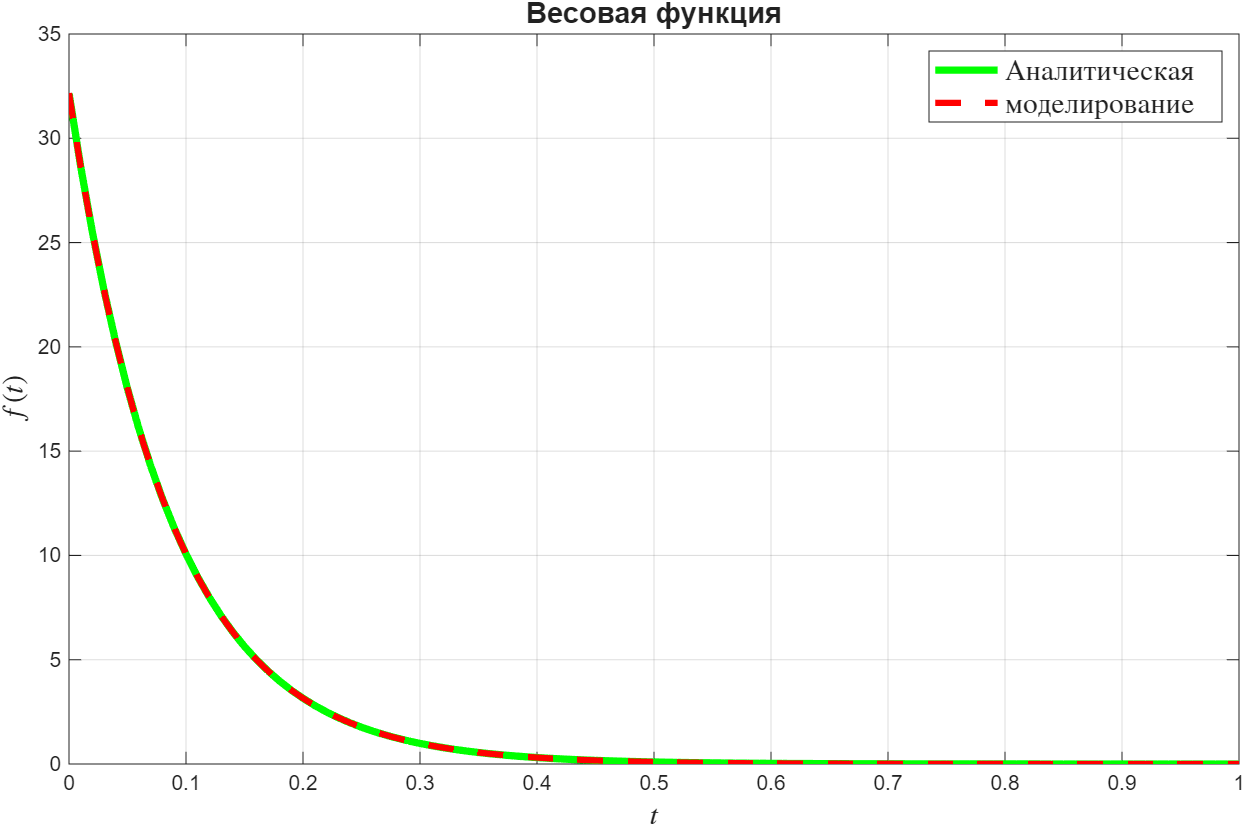
\includegraphics[width=0.84\linewidth]{images/Figure_5_1_1.png}
    \caption{График сравнения весовых характеристик}
    \label{fig:placeholder}
\end{figure}

\begin{figure}[H]
    \centering
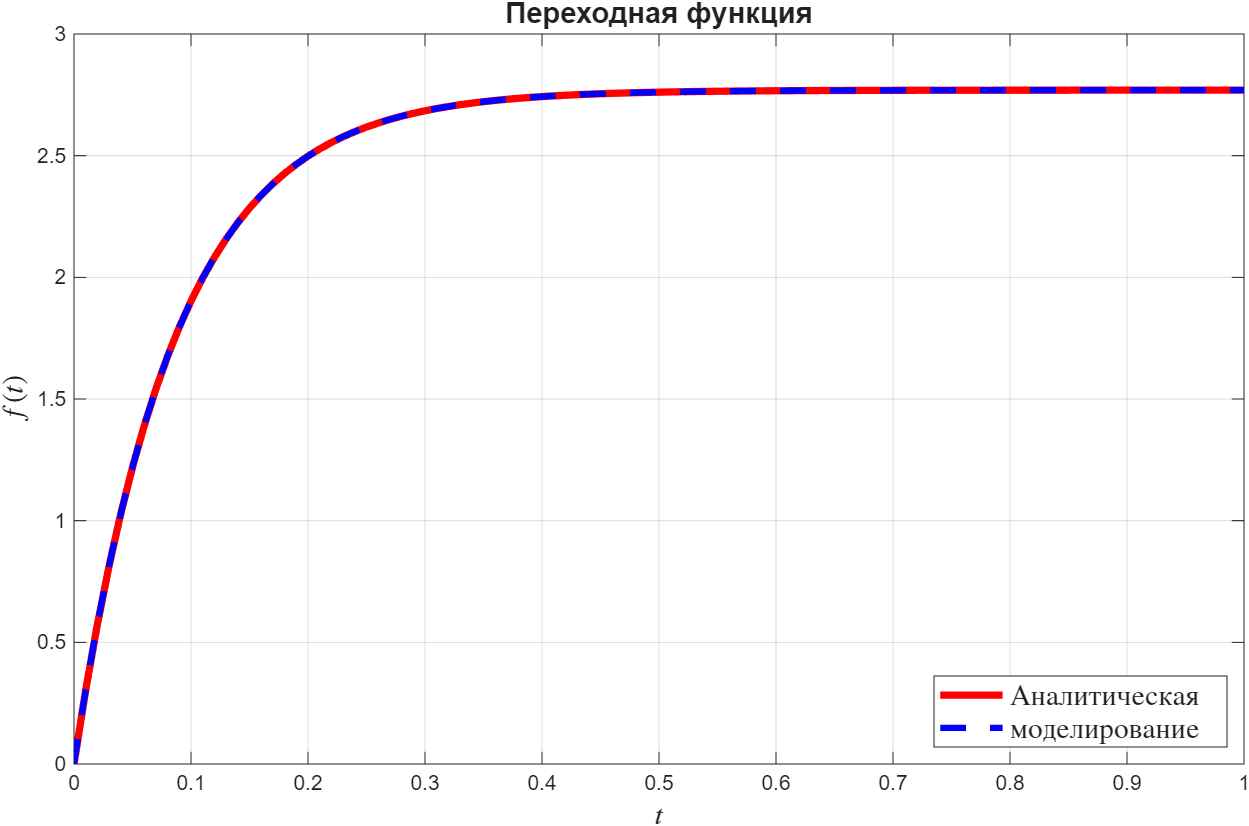
\includegraphics[width=0.84\linewidth]{images/Figure_5_1_2.png}
    \caption{График сравнения переходных характеристик}
    \label{fig:placeholder}
\end{figure}

\begin{figure}[H]
    \centering
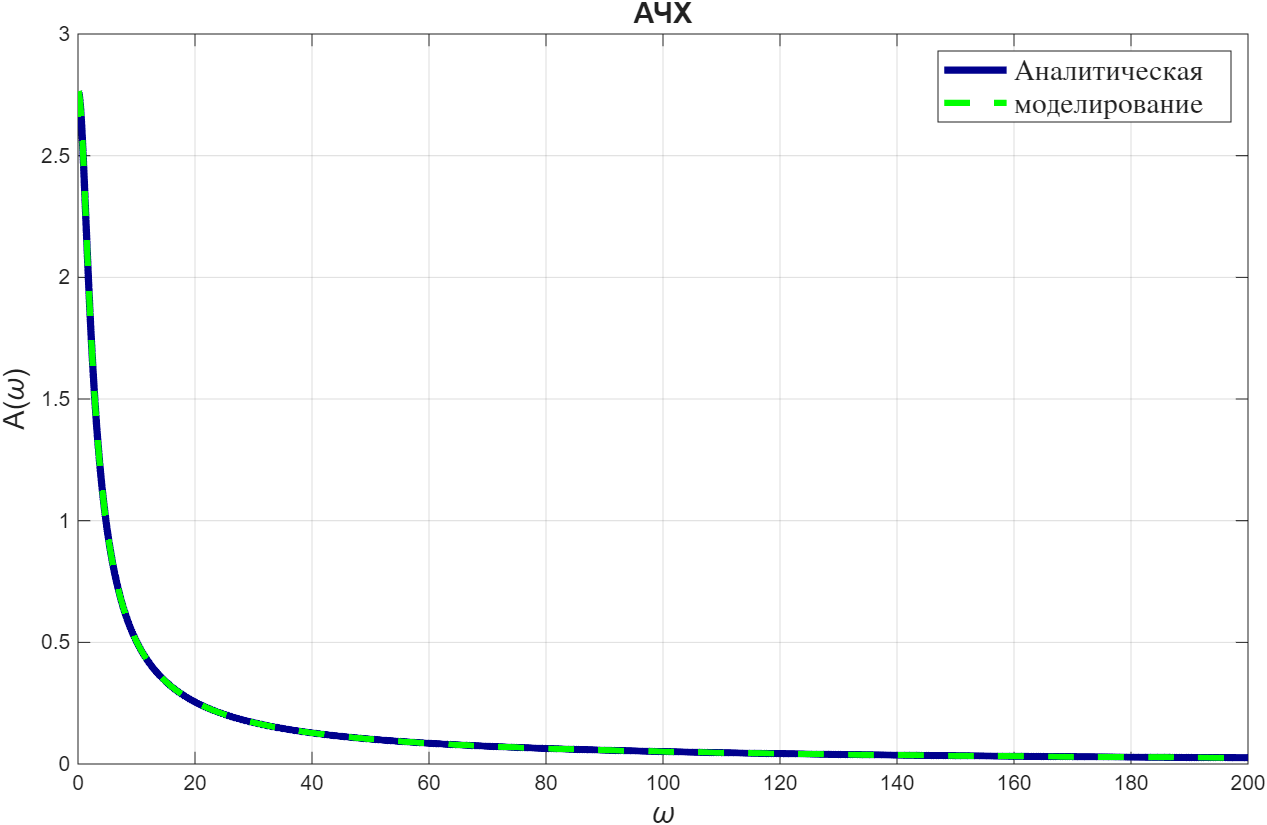
\includegraphics[width=0.84\linewidth]{images/Figure_5_1_3.png}
    \caption{График сравнения АЧХ}
    \label{fig:placeholder}
\end{figure}

\begin{figure}[H]
    \centering
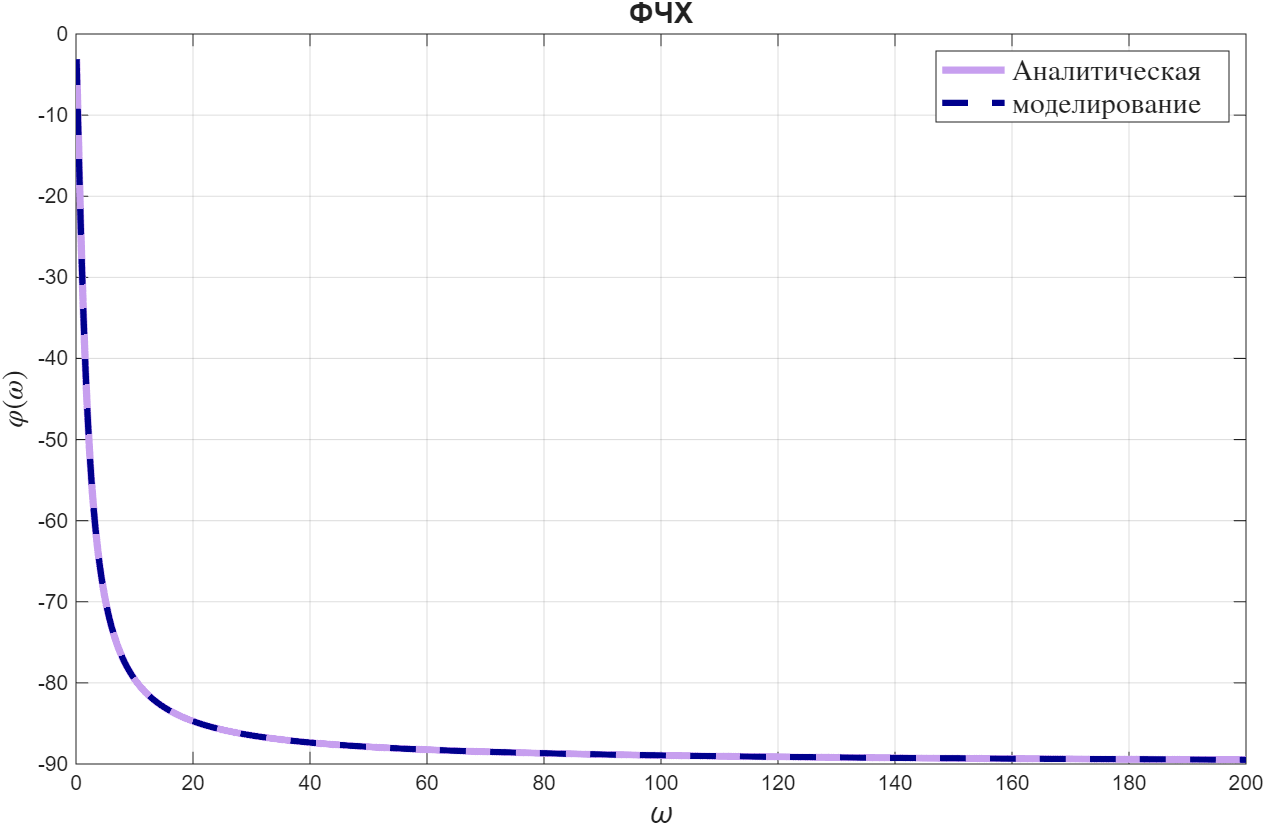
\includegraphics[width=0.84\linewidth]{images/Figure_5_1_4.png}
    \caption{График сравнения ФЧХ}
    \label{fig:placeholder}
\end{figure}

\begin{figure}[H]
    \centering
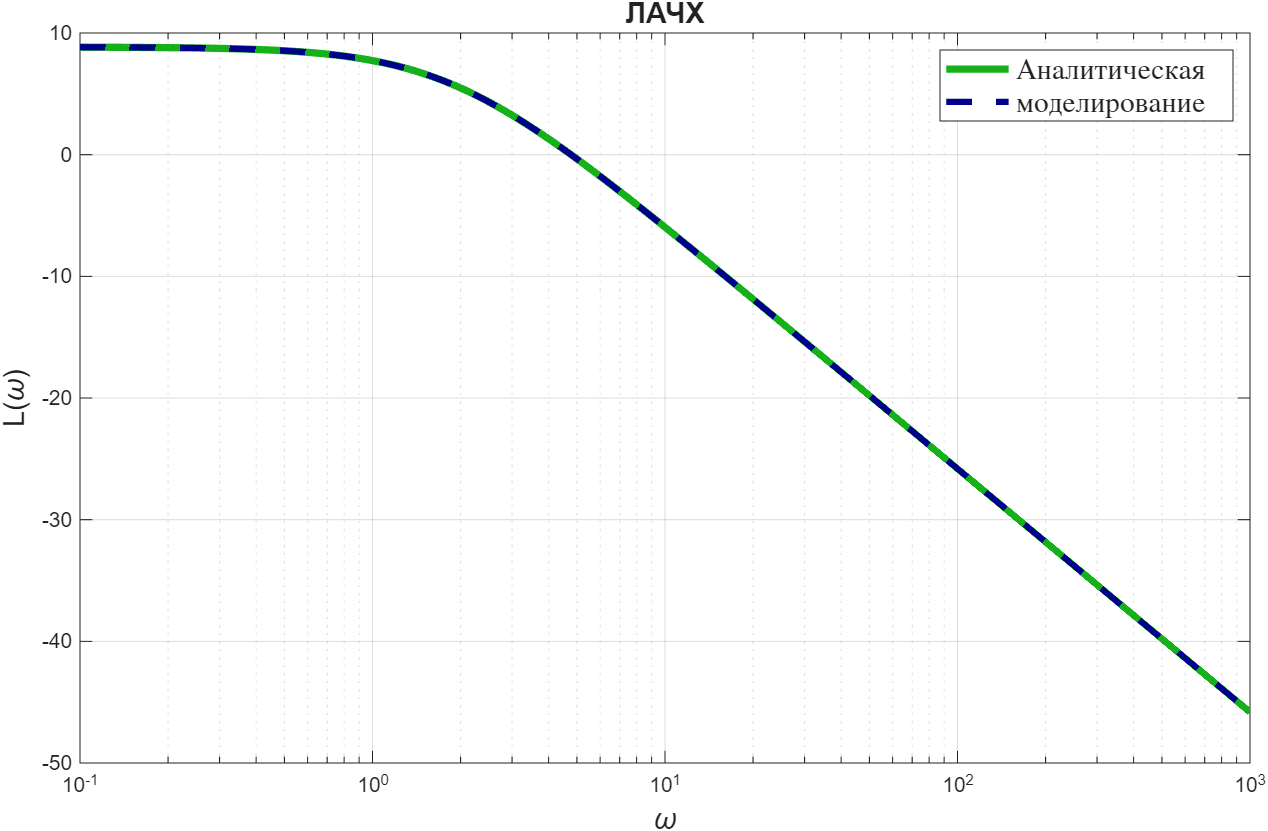
\includegraphics[width=0.84\linewidth]{images/Figure_5_1_5.png}
    \caption{График сравнения ЛАЧХ}
    \label{fig:placeholder}
\end{figure}

\begin{figure}[H]
    \centering
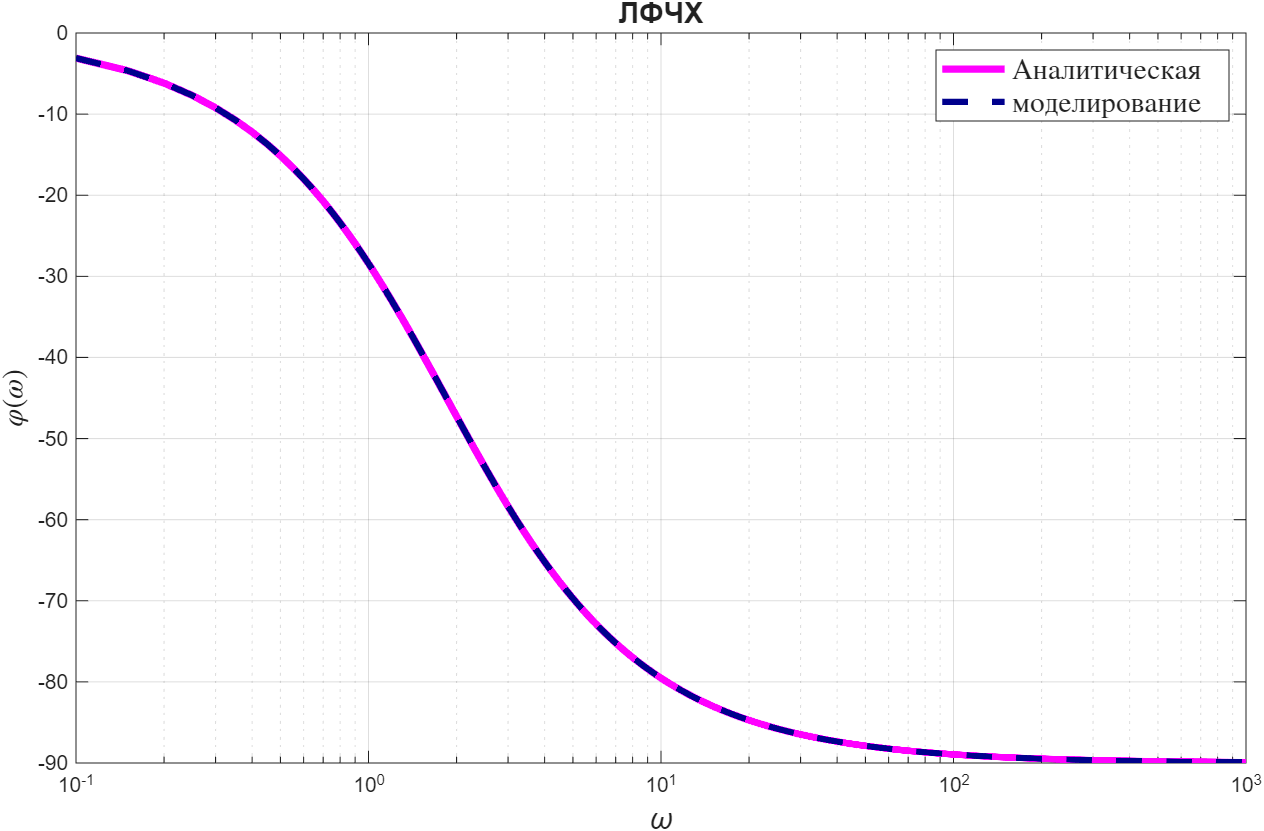
\includegraphics[width=0.84\linewidth]{images/Figure_5_1_6.png}
    \caption{График сравнения ЛФЧХ}
    \label{fig:placeholder}
\end{figure}

Как можно заметить, что графики полностью совпадают, на предложенных промежутках, что даёт понять, что все проделанные вычисления верны.

\subsection{Выводы}

Двигатель постоянного тока является реальным усилительным звеном первого порядка. Результаты моделирования полностью соответствуют аналитическим, что подтверждает корректность расчётов.


\section{Объект 2. ДПТ 2.0}

\subsection{Исходные данные}
\begin{center}
\begin{tabular}{|c|c|}
\hline
Параметр & Значение \\ \hline
$k_m$ & 0,3611 \,Н·м/А \\ \hline
$k_e$&0,3611 \,B·c \\ \hline
$J$ & 0,0024 \,кг·м$^2$ \\ \hline
$R$ & 4,6775 \,Ом \\ \hline
$L$ & 1.1056 \,Гн \\ \hline
\end{tabular}
\end{center}

Вход — напряжение $U(t)$, выход — угловая скорость $\omega(t)$.

\subsection{Вывод передаточной функции}

Даны уравнения двигателя постоянного тока независимого возбуждения:

\[
J\dot{\omega} = M, \quad 
M = k_m I, \quad 
I = \frac{U + \varepsilon}{R}, \quad 
\varepsilon = \varepsilon_i + \varepsilon_s, \quad 
\varepsilon_i = -k_e \omega, \quad 
\varepsilon_s = -L \dot{I}.
\]

Пользуясь приведенными соотношениями, получим ДУ системы.

\[
\begin{cases} 
J\dot{\omega} = k_m I \\ 
I = \dfrac{U - k_e \omega - L\dot{I}}{R} 
\end{cases}
\]

\[
\begin{cases} 
\dot{\omega} = \dfrac{k_m}{J}I \\ 
\dot{I} = \dfrac{1}{L}U - \dfrac{k_e}{L}\omega - \dfrac{R}{L}I 
\end{cases}
\]


\[
\begin{cases} 
\ddot{\omega} = \dfrac{k_m}{J}\dot{I} \\ 
\dot{I} = \dfrac{1}{L}U - \dfrac{k_e}{L}\omega - \dfrac{R}{L}I 
\end{cases}
\]


\[
\ddot{\omega} = \dfrac{k_m}{J}\left(\dfrac{1}{L}U - \dfrac{k_e}{L}\omega - \dfrac{R}{L}I\right)
\]



\[
\ddot{\omega} = \dfrac{k_m}{J}\left(\dfrac{1}{L}U - \dfrac{k_e}{L}\omega - \dfrac{R}{L}\cdot \dfrac{J}{k_m}\dot{\omega}\right)
\]

\[
\ddot{\omega} = \dfrac{k_m}{JL}U - \dfrac{k_m k_e}{JL}\omega - \dfrac{R}{L}\dot{\omega}
\]

\[
\ddot{\omega} + \dfrac{R}{L}\dot{\omega} + \dfrac{k_m k_e}{JL}\omega = \dfrac{k_m}{JL}U
\]


\[
\left(p^2 + \dfrac{R}{L}p + \dfrac{k_m k_e}{JL}\right)\omega = \dfrac{k_m}{JL}U
\]

\[
\omega = \frac{\dfrac{k_m}{JL}}{p^2 + \dfrac{R}{L}p + \dfrac{k_m k_e}{JL}} \; U
\]

\[
W(s) = \frac{k_m}{JLs^2 + JRs + k_m k_e}
\]

\[
W(s) = \dfrac{k_m}{JLs^2 + JRs + k_m k_e}
\]

\[
W(s) = \dfrac{\dfrac{1}{k_e}}{\dfrac{JLs^2}{k_m k_e} + \dfrac{JRs}{k_m k_e} + 1}
\]

\[
K=\dfrac{b_0}{a_0}=\dfrac{\dfrac{k_m}{JL}}{\dfrac{k_mk_e}{JL}}=\dfrac{1}{k_e}, \quad T=\sqrt{\dfrac{a_2}{a_0}}=\sqrt{\dfrac{JL}{k_mk_e}},\]
\[
\xi=\dfrac{a_1}{2\sqrt{a_0a_2}}=\dfrac{\dfrac{R}{L}}{2\sqrt{\dfrac{k_mk_e}{JL}}}=\dfrac{RJ}{2\sqrt{k_mk_eLJ}}
\]

$$
W(p) = \frac{K}{T^2 p^2 + 2 \xi T p + 1}.
$$

$$0\leq\xi\approx0.3018\leq1$$

\textbf{Тип звена:} Колебательное звено


\subsection{Аналитические выражения временны́х характеристик}


\textbf{Весовая характеристика} $w(t)$:
$$w(t)=\mathcal{L}^{-1}\{ W(s)\}$$

$$w(t)=\mathcal{L}^{-1}\left\{ \frac{K}{T^2 s^2 + 2 \xi T s + 1}\right\}$$

$$w(t)=\mathcal{L}^{-1}\left\{ \dfrac{K}{T^2}\cdot\frac{1}{s^2 + \dfrac{2 \xi s}{T} + \dfrac{1}{T^2}}\right\}$$

$$w(t)=\mathcal{L}^{-1}\left\{ \dfrac{K}{T^2}\cdot\frac{1}{\left(s + \dfrac{ \xi }{T}\right)^2 + \left(\dfrac{\sqrt{1-\xi^2}}{T}\right)^2}\right\}$$

$$w(t)=\mathcal{L}^{-1}\left\{ \dfrac{K}{T\sqrt{1-\xi^2}}\cdot\frac{\dfrac{\sqrt{1-\xi^2}}{T}}{\left(s + \dfrac{ \xi }{T}\right)^2 + \left(\dfrac{\sqrt{1-\xi^2}}{T}\right)^2}\right\}$$

$$w(t)=\dfrac{K}{T\sqrt{1-\xi^2}}\mathcal{L}^{-1}\left\{\frac{\dfrac{\sqrt{1-\xi^2}}{T}}{\left(s + \dfrac{ \xi }{T}\right)^2 + \left(\dfrac{\sqrt{1-\xi^2}}{T}\right)^2}\right\}$$

$$w(t)=\dfrac{K}{T\sqrt{1-\xi^2}}\exp\left(-\dfrac{\xi}{T}t\right)\sin\left(\dfrac{\sqrt{1-\xi^2}}{T}t\right)$$







\textbf{Переходная характеристика} $h(t)$:
\[
h(t) = \mathcal{L}^{-1}\!\left\{ \frac{W(s)}{s} \right\}
     = \mathcal{L}^{-1}\!\left\{ \frac{K}{s(T^2 s^2 + 2\xi T s + 1)} \right\}.
\]

\[
h(t)=\mathcal{L}^{-1}\!\left\{\frac{K}{s(T^2 s^2 + 2\xi T s + 1)}\right\}
     = \frac{K}{T^2} \cdot\mathcal{L}^{-1}\!\left\{ \frac{1}{s\left(\left(s + \dfrac{ \xi }{T}\right)^2 + \left(\dfrac{\sqrt{1-\xi^2}}{T}\right)^2\right)}\right\}
\]

\[
h(t)=\mathcal{L}^{-1}\!\left\{\frac{K}{s(T^2 s^2 + 2\xi T s + 1)}\right\}
     = \frac{K}{T^2} \cdot\mathcal{L}^{-1}\!\left\{ \dfrac{A}{s}+\frac{Bs+C}{\left(s + \dfrac{ \xi }{T}\right)^2 + \left(\dfrac{\sqrt{1-\xi^2}}{T}\right)^2}\right\}
\]

\[
1=A\left(\left(s + \dfrac{ \xi }{T}\right)^2 + \left(\dfrac{\sqrt{1-\xi^2}}{T}\right)^2\right)+\left(Bs+C\right)s
\]
\vspace{0.5cm}

Раскроем и приравняем коэффициенты при одинаковых степенях $s$:
\begin{align*}
s^2: &\quad A + B = 0 \\
s^1: &\quad 2\dfrac{\xi}{T} A + C = 0 \\
s^0: &\quad A\left(\left(\dfrac{\xi}{T}\right)^2 + \left(\frac{\sqrt{1-\xi^2}}{T}\right)^2\right) = 1
\end{align*}

\[
A = \frac{1}{\left(\dfrac{\xi}{T}\right)^2 + \left(\dfrac{\sqrt{1-\xi^2}}{T}\right)^2}  = T^2
\]
\[
B = -A = -T^2
\]
\[
C = -2\alpha A = -2\dfrac{\xi}{T} T^2 = -2\xi T
\]

\[
h(t)= \frac{K}{T^2} \cdot\mathcal{L}^{-1}\!\left\{ \dfrac{T^2}{s}+\frac{-T^2s-2\xi T}{\left(s + \dfrac{ \xi }{T}\right)^2 + \left(\dfrac{\sqrt{1-\xi^2}}{T}\right)^2}\right\}
\]

$$\dfrac{T^2}{s}+\frac{-T^2s-2\xi T}{\left(s + \dfrac{ \xi }{T}\right)^2 + \left(\dfrac{\sqrt{1-\xi^2}}{T}\right)^2}=$$
 $$=\dfrac{T^2}{s}-\frac{T^2\left(s+\dfrac{\xi}{T}\right)}{\left(s + \dfrac{ \xi }{T}\right)^2 + \left(\dfrac{\sqrt{1-\xi^2}}{T}\right)^2}+$$
 $$+\frac{\dfrac{\xi}{T}}{\left(s + \dfrac{ \xi }{T}\right)^2 + \left(\dfrac{\sqrt{1-\xi^2}}{T}\right)^2}-\frac{2\xi T}{\left(s + \dfrac{ \xi }{T}\right)^2 + \left(\dfrac{\sqrt{1-\xi^2}}{T}\right)^2}$$


\[
h(t) = K \left[ 1 
- T^2 e^{-\frac{\xi}{T}t} \left( 
\cos\!\left( \frac{\sqrt{1-\xi^2}}{T} t \right)
+ \frac{\xi}{\sqrt{1-\xi^2}} 
\sin\!\left( \frac{\sqrt{1-\xi^2}}{T} t \right)
\right) \right].
\]















\subsection{Аналитические выражения частотных характеристик}


Частотная передаточная функция:
\[
W(j\omega) = \frac{K}{T^2(j\omega)^2 + 2T\xi(j\omega) + 1} 
           = \frac{K}{1 - T^2\omega^2 + 2T\xi j\omega}.
\]

Умножим числитель и знаменатель на комплексно-сопряжённое к знаменателю:
\[
W(j\omega) = \frac{K(1 - T^2\omega^2 - 2T\xi j\omega)}{(1 - T^2\omega^2 + 2T\xi j\omega)(1 - T^2\omega^2 - 2T\xi j\omega)} \]
                  
\[W(j\omega) = \frac{K(1 - T^2\omega^2)}{(1 - T^2\omega^2)^2 + 4T^2\xi^2\omega^2}-\frac{2KT\xi j\omega}{(1 - T^2\omega^2)^2 + 4T^2\xi^2\omega^2}\]


Выделим действительную $P(\omega)$ и мнимую $Q(\omega)$ части:
\[
P(\omega) = \frac{K(1 - T^2\omega^2)}{(1 - T^2\omega^2)^2 + 4T^2\xi^2\omega^2}
\qquad
Q(\omega) = -\frac{2KT\xi \omega}{(1 - T^2\omega^2)^2 + 4T^2\xi^2\omega^2}
\]

\vspace{0.5cm}

\textbf{Амплитудно-частотная характеристика:}

\[A(\omega) = \sqrt{P(\omega)^2 + Q(\omega)^2} \]
         \[ A(\omega)= \sqrt{
             \left(\frac{K(1 - T^2\omega^2)}
                        {(1 - T^2\omega^2)^2 + 4T^2\xi^2\omega^2}\right)^{\!2}
             + \left(\frac{-2KT\xi\omega}
                           {(1 - T^2\omega^2)^2 + 4T^2\xi^2\omega^2}\right)^{\!2}
             } \]
          \[A(\omega)= \frac{K}{(1 - T^2\omega^2)^2 + 4T^2\xi^2\omega^2}
             \sqrt{(1 - T^2\omega^2)^2 + 4T^2\xi^2\omega^2} \]
          \[A(\omega)= \frac{K}{\sqrt{(1 - T^2\omega^2)^2 + 4T^2\xi^2\omega^2}}\]

\vspace{0.5cm}

\textbf{Фазо-частотная характеристика:}

\[\varphi(\omega) = \operatorname{atan2}\!\big(Q(\omega),\, P(\omega)\big) \]
                \[\varphi(\omega)= \operatorname{atan2}\!\left(
                   -\frac{2KT\xi\omega}
                         {(1 - T^2\omega^2)^2 + 4T^2\xi^2\omega^2},\;
                   \frac{K(1 - T^2\omega^2)}
                         {(1 - T^2\omega^2)^2 + 4T^2\xi^2\omega^2}
                   \right) \]
              \[\varphi(\omega)= \operatorname{atan2}\!\big(-2T\xi\omega,\; 1 - T^2\omega^2\big)\]

\[\varphi(\omega) = -\arctan\left(\frac{2\xi T\omega}{1 - T^2\omega^2}\right)\]

\vspace{0.5cm}

\textbf{Логарифмическая амплитудно-частотная характеристика:}
\[
L(\omega) = 20\lg\!\big(A(\omega)\big) 
          = 20\lg\!\left(
            \frac{K}{\sqrt{(1 - T^2\omega^2)^2 + 4T^2\xi^2\omega^2}}
            \right).
\]



\subsection{Моделирование в MATLAB}

\begin{figure}[H]
    \centering
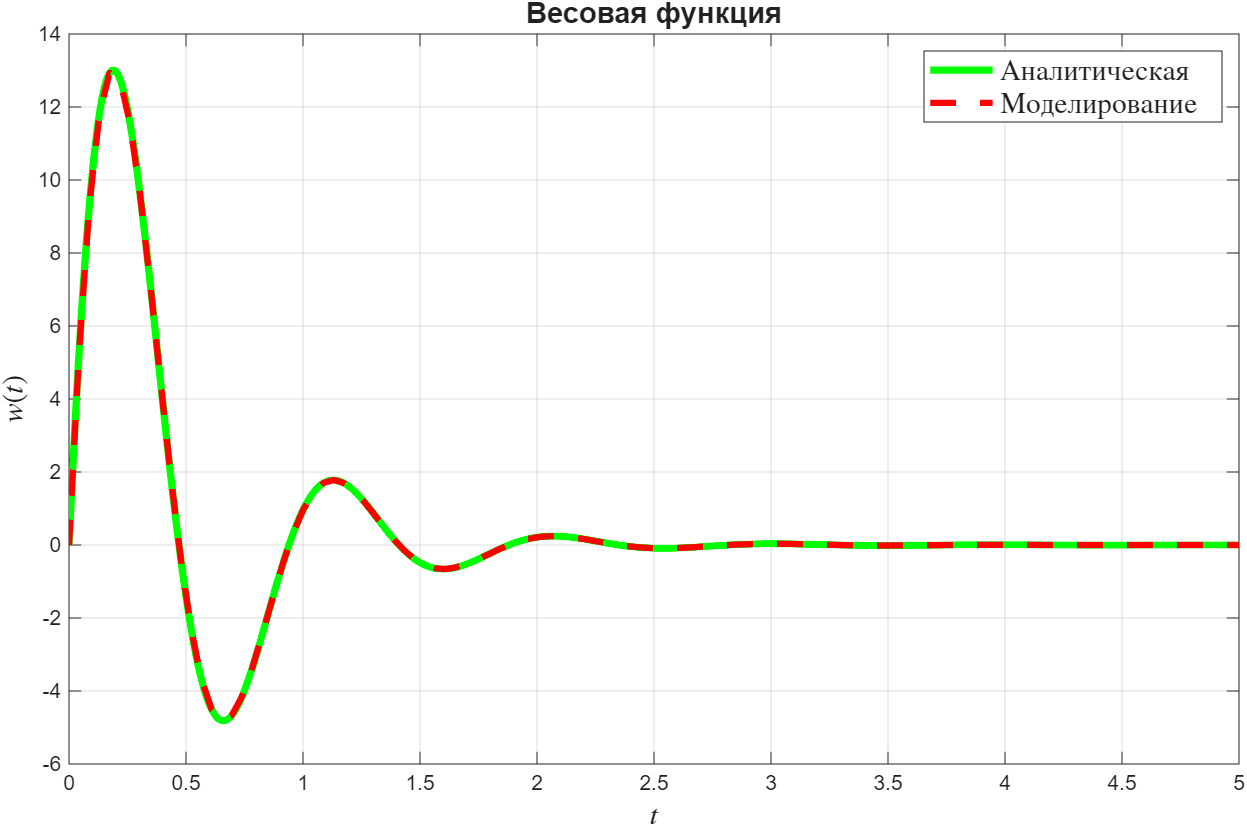
\includegraphics[width=0.84\linewidth]{images/Figure_5_2_1.png}
    \caption{График сравнения весовых характеристик}
    \label{fig:placeholder}
\end{figure}

\begin{figure}[H]
    \centering
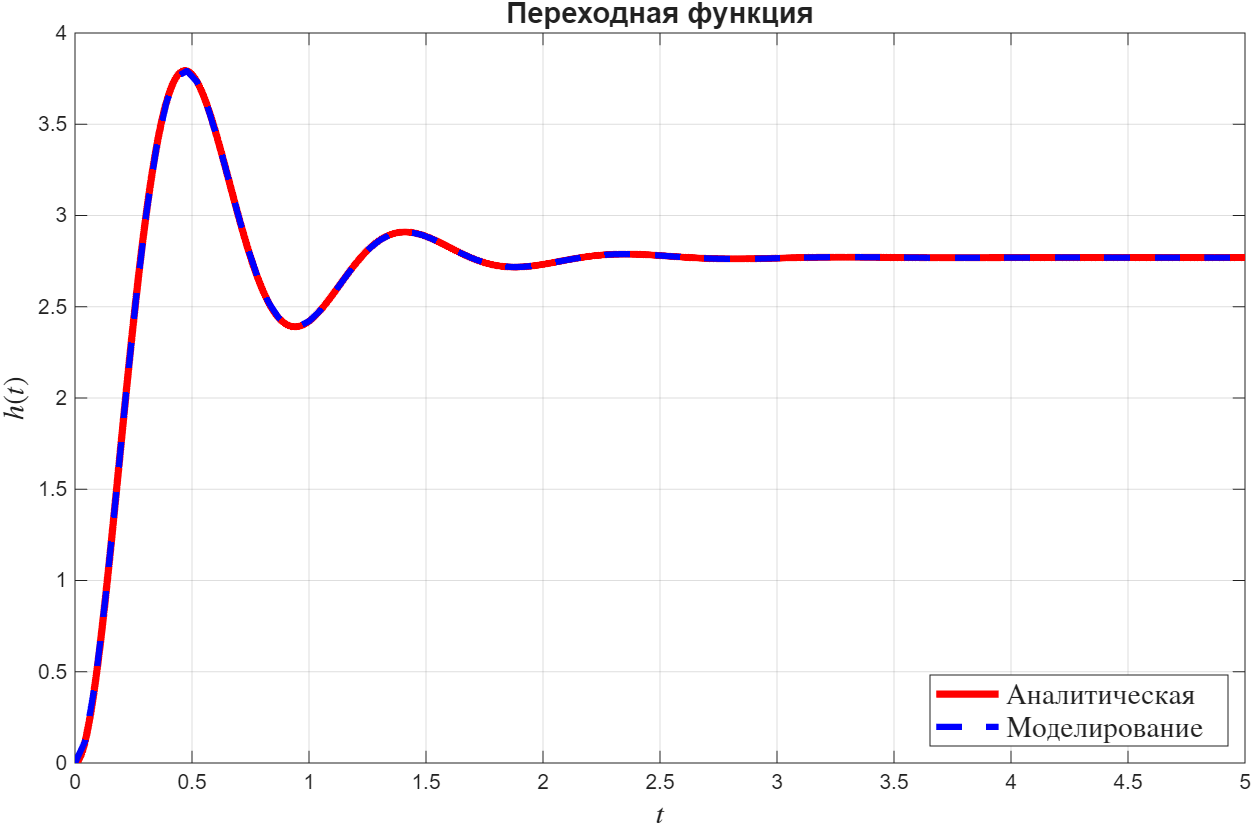
\includegraphics[width=0.84\linewidth]{images/Figure_5_2_2.png}
    \caption{График сравнения переходных характеристик}
    \label{fig:placeholder}
\end{figure}

\begin{figure}[H]
    \centering
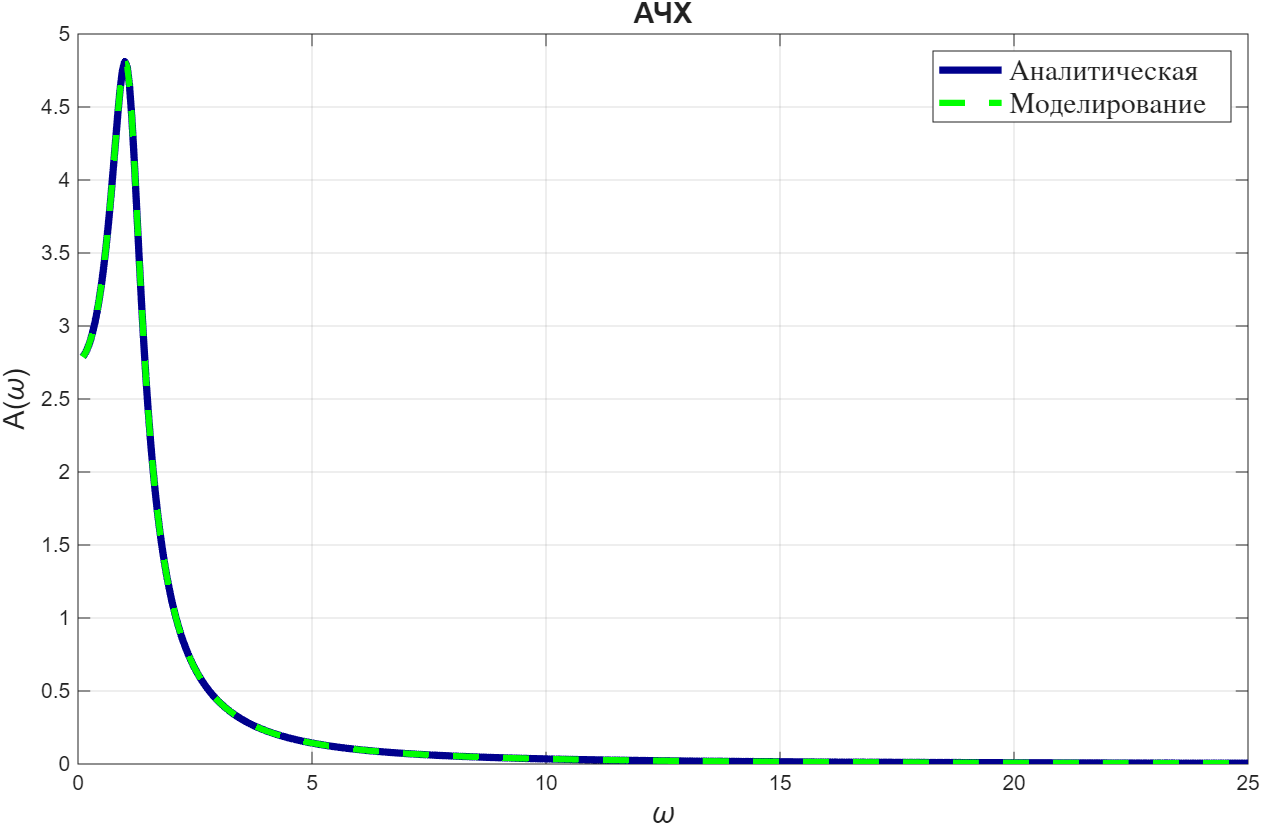
\includegraphics[width=0.84\linewidth]{images/Figure_5_2_3.png}
    \caption{График сравнения АЧХ}
    \label{fig:placeholder}
\end{figure}

\begin{figure}[H]
    \centering
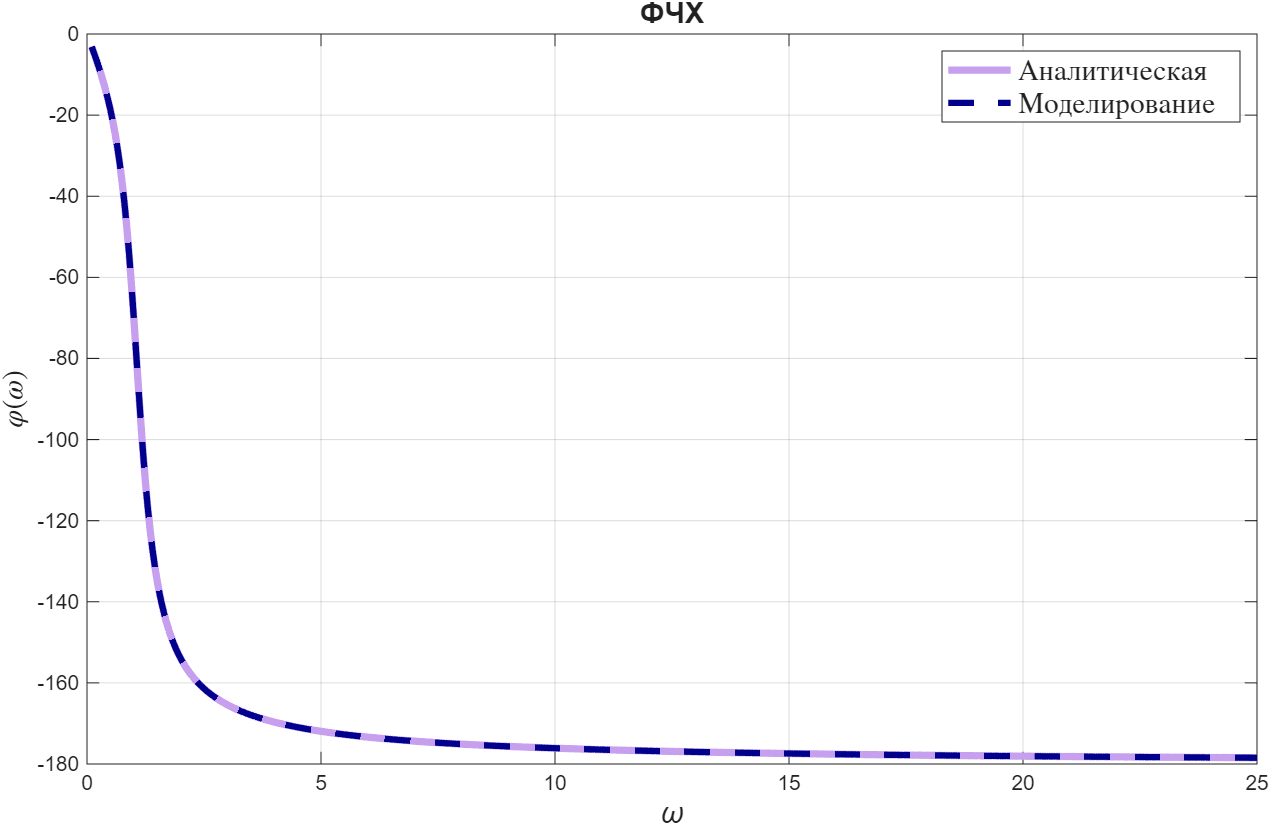
\includegraphics[width=0.84\linewidth]{images/Figure_5_2_4.png}
    \caption{График сравнения ФЧХ}
    \label{fig:placeholder}
\end{figure}

\begin{figure}[H]
    \centering
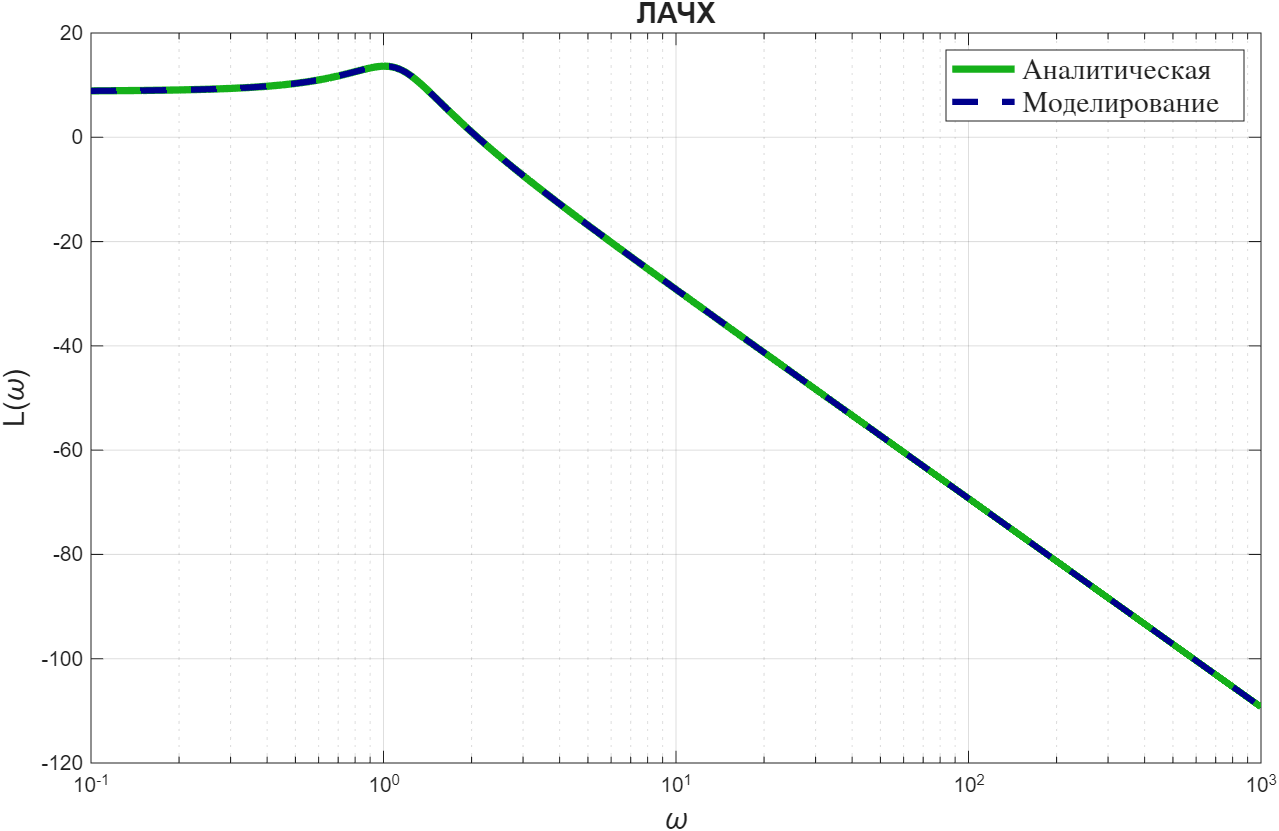
\includegraphics[width=0.84\linewidth]{images/Figure_5_2_5.png}
    \caption{График сравнения ЛАЧХ}
    \label{fig:placeholder}
\end{figure}

\begin{figure}[H]
    \centering
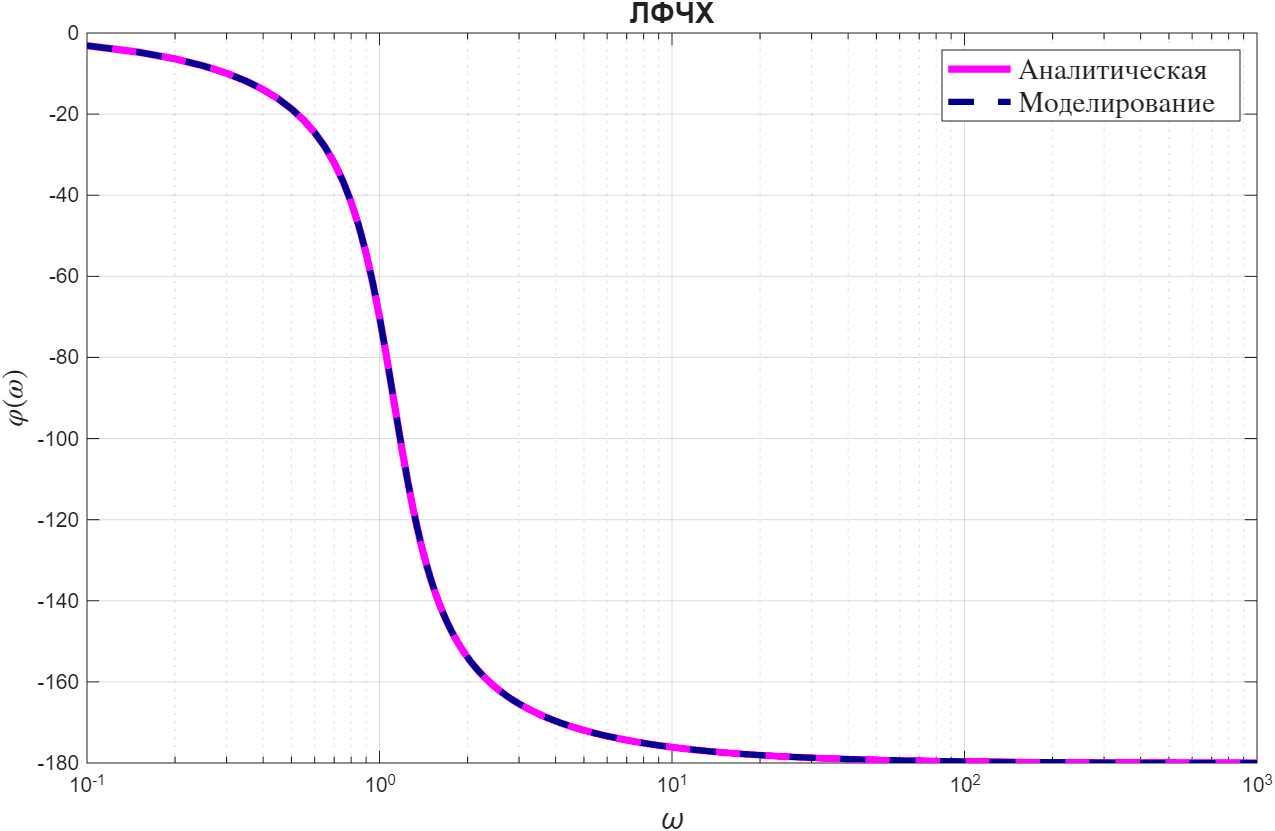
\includegraphics[width=0.84\linewidth]{images/Figure_5_2_6.png}
    \caption{График сравнения ЛФЧХ}
    \label{fig:placeholder}
\end{figure}

Как можно заметить, что графики полностью совпадают, на предложенных промежутках, что даёт понять, что все проделанные вычисления верны.

\subsection{Выводы}

Двигатель с учётом индуктивности является колебательным звеном. Это отличает его от апериодического звена (Объект 1), демонстрируя влияние индуктивности на динамику системы: появление колебательного характера переходных процессов. Результаты моделирования подтверждают корректность вычислений.













\section{Объект 3. Конденсируй-умножай}

\subsection{Исходные данные}
\begin{center}
\begin{tabular}{|c|c|}
\hline
Параметр & Значение \\ \hline
$C$ — ёмкость конденсатора & 434 мкФ = $4.34 \times 1^{-4}$ Ф \\
\hline
\end{tabular}
\end{center}

Входом объекта считаем $I(t)$, а выходом $U(t)$.

\subsection{Вывод передаточной функции}

\[
I(t) = C \frac{dU(t)}{dt} \]
\[
\frac{1}{C} I(t)=\frac{dU(t)}{dt}
\]
\[
\dfrac{p}{C}I=U
\]
\[
W(s) = \frac{U(s)}{I(s)} = \frac{1}{C s}= \frac{C^{-1}}{s}
\]


\textbf{Тип звена:} Идеальное интегрирующее звено

\subsection{Аналитические выражения временны́х характеристик}

\textbf{Весовая характеристика} $w(t)$:
\[
w(t)=\mathcal{L}^{-1}\left\{ W(s) \right\}=\mathcal{L}^{-1}\left\{ \frac{C^{-1}}{s} \right\}=\dfrac{1}{C}
\]
\textbf{Переходная характеристика} $h(t)$:
\[
h(t)=\mathcal{L}^{-1}\left\{\dfrac{W(s)}{s}\right\}=\mathcal{L}^{-1}\left\{\frac{C^{-1}}{s^{2}}\right\}=\dfrac{t}{C}
\]

\subsection{Аналитические выражения частотных характеристик}
Частотная передаточная функция:
\[
W(j\omega)=\dfrac{1}{j\omega C}=-\dfrac{j}{\omega C}
\]
Выделим действительную $P(\omega)$ и мнимую $Q(\omega)$ части:
\[
P(\omega)=0,\quad Q(\omega)=-\dfrac{j}{\omega C}
\]

\textbf{Амплитудно-частотная характеристика:}
\[
A(\omega)=\sqrt{P(\omega)^{2} + Q(\omega)^{2}}=\sqrt{\left(-\dfrac{1}{\omega C}\right)^{2}}=\dfrac{1}{\omega C}
\]

\textbf{Фазо-частотная характеристика:}
\[
\varphi(\omega)=\arctan2(Q(\omega), P(\omega))=\arctan2\left(-\dfrac{1}{\omega C}, 0\right)=\dfrac{\pi}{2}
\]

\textbf{Логарифмическая амплитудно-частотная характеристика:}
\[
L(\omega)=20\lg(A(\omega))=20\lg\left(\dfrac{1}{\omega C}\right)
\]



\subsection{Моделирование в MATLAB}

\begin{figure}[H]
    \centering
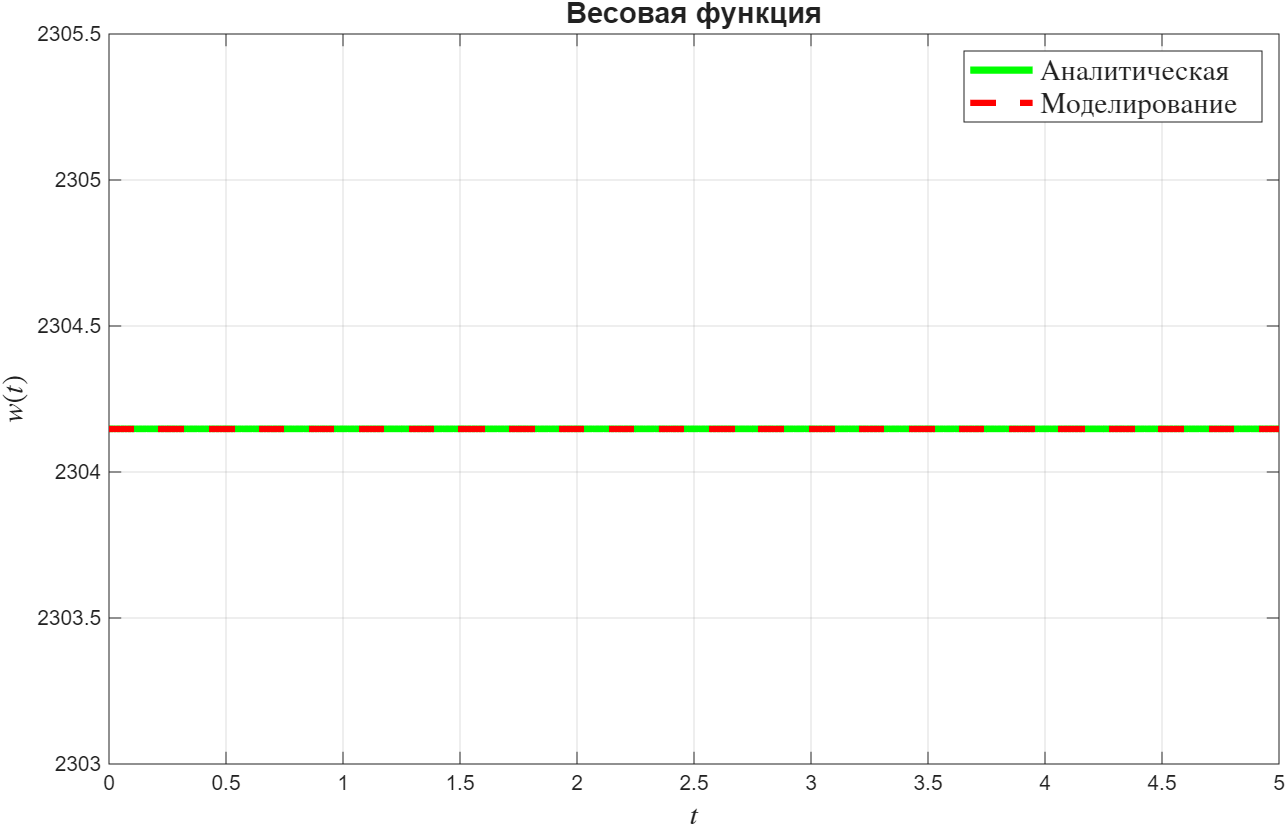
\includegraphics[width=0.84\linewidth]{images/Figure_5_3_1.png}
    \caption{График сравнения весовых характеристик}
    \label{fig:placeholder}
\end{figure}

\begin{figure}[H]
    \centering
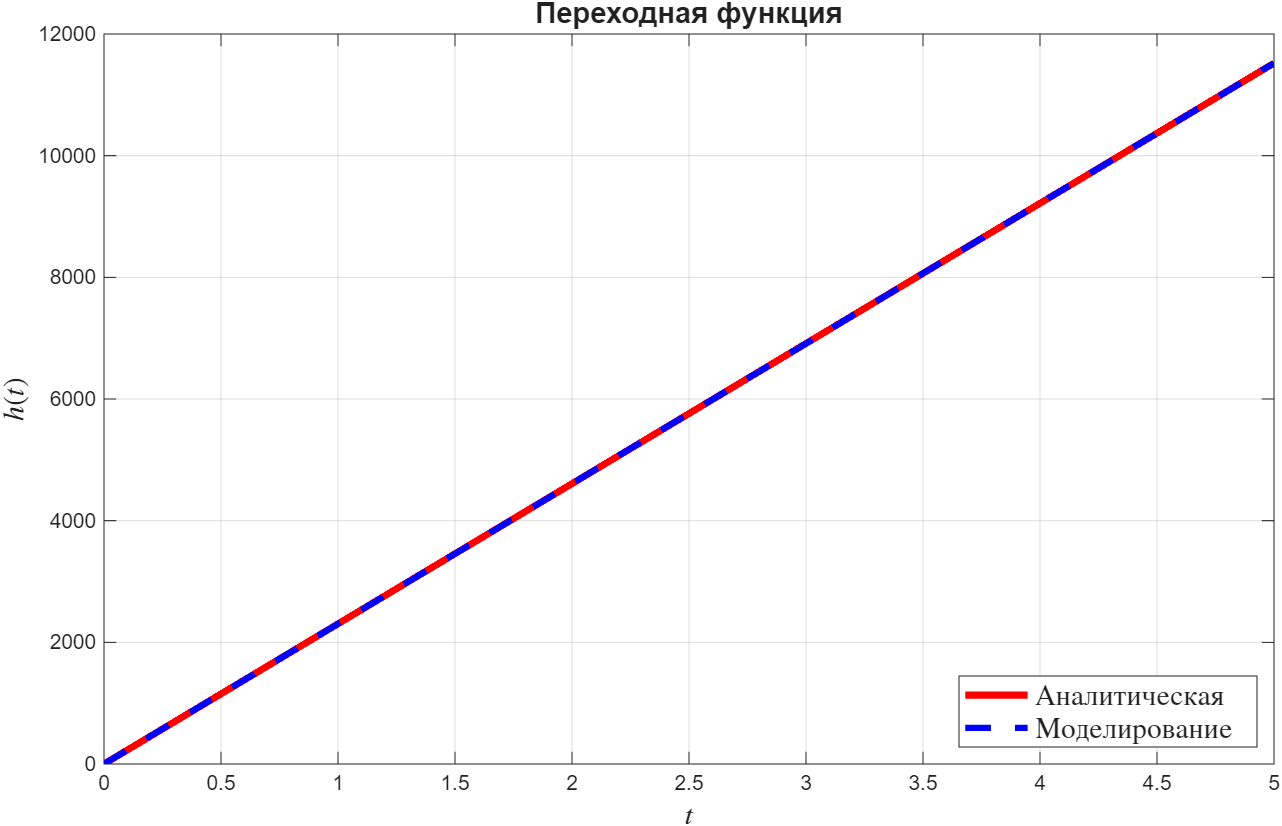
\includegraphics[width=0.84\linewidth]{images/Figure_5_3_2.png}
    \caption{График сравнения переходных характеристик}
    \label{fig:placeholder}
\end{figure}

\begin{figure}[H]
    \centering
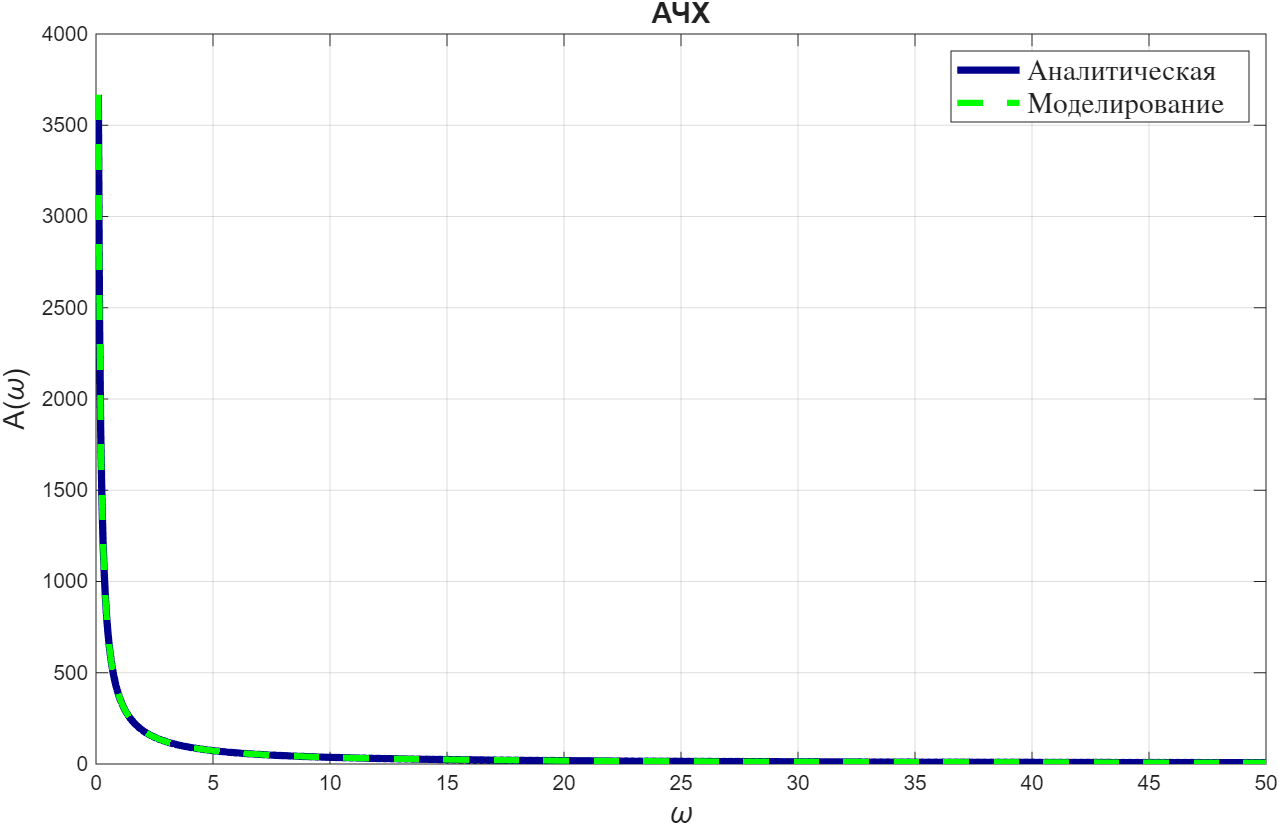
\includegraphics[width=0.84\linewidth]{images/Figure_5_3_3.png}
    \caption{График сравнения АЧХ}
    \label{fig:placeholder}
\end{figure}

\begin{figure}[H]
    \centering
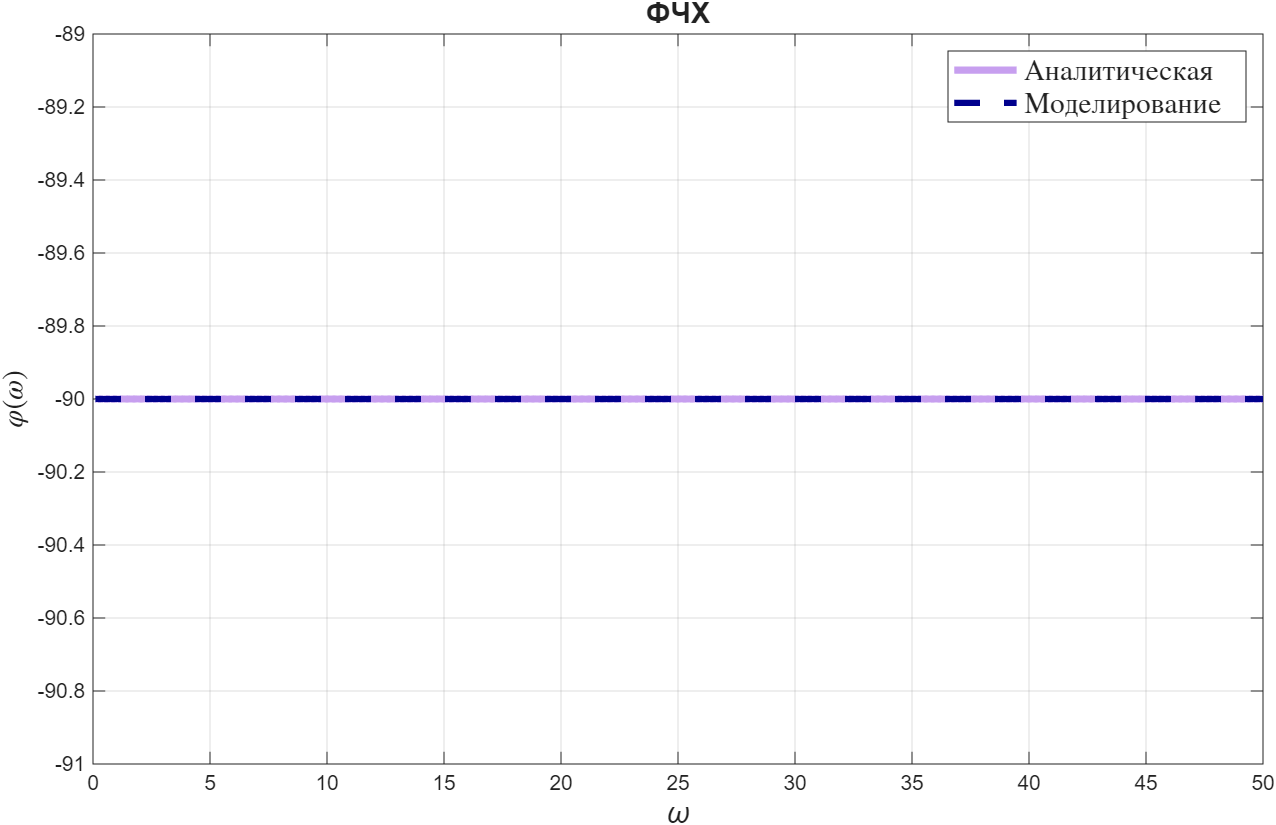
\includegraphics[width=0.84\linewidth]{images/Figure_5_3_4.png}
    \caption{График сравнения ФЧХ}
    \label{fig:placeholder}
\end{figure}

\begin{figure}[H]
    \centering
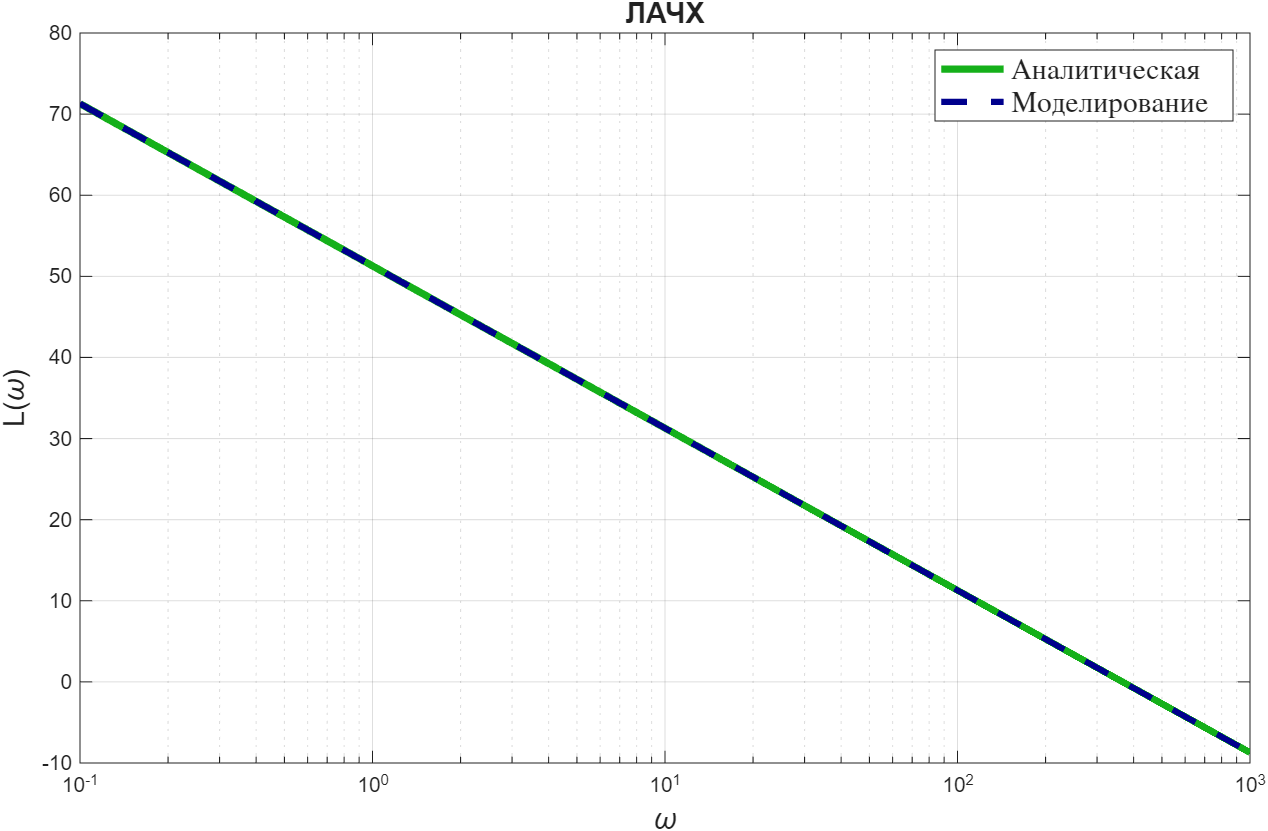
\includegraphics[width=0.84\linewidth]{images/Figure_5_3_5.png}
    \caption{График сравнения ЛАЧХ}
    \label{fig:placeholder}
\end{figure}

\begin{figure}[H]
    \centering
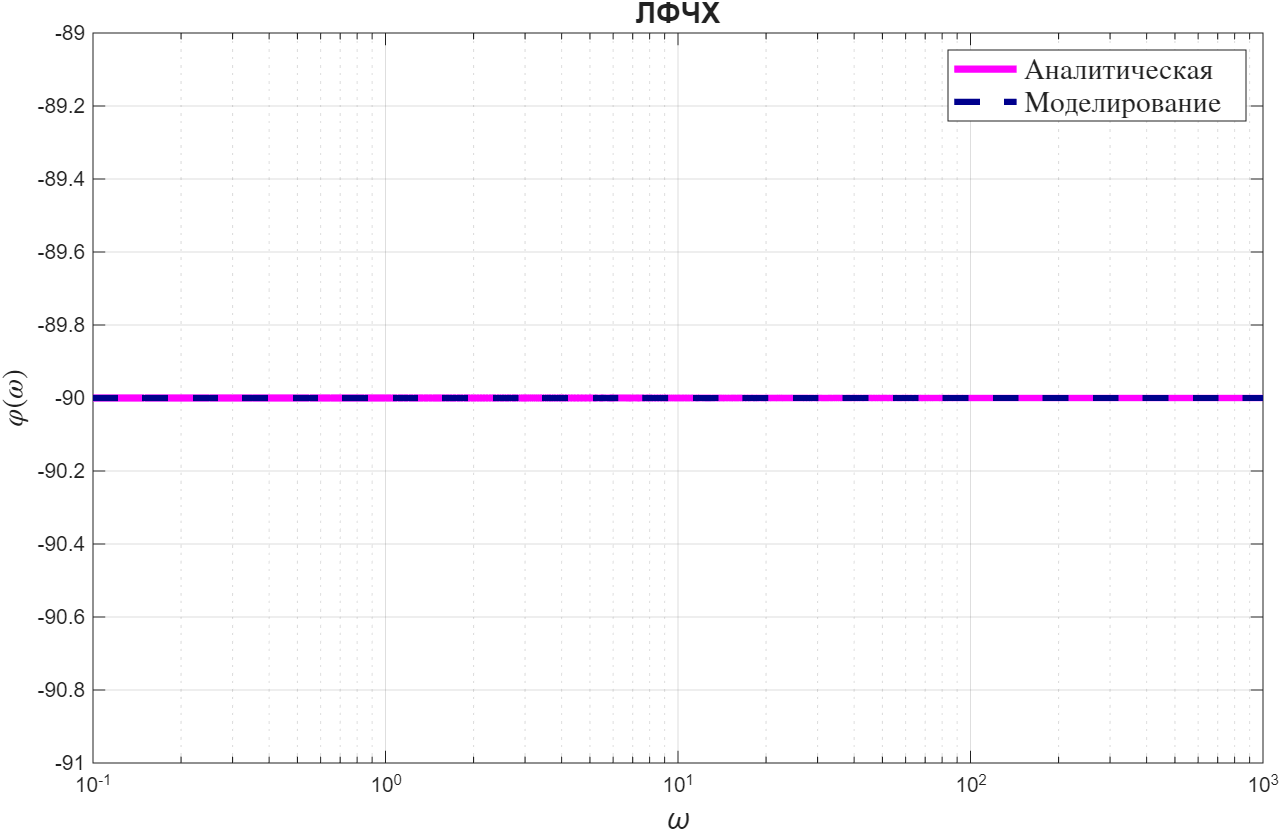
\includegraphics[width=0.84\linewidth]{images/Figure_5_3_6.png}
    \caption{График сравнения ЛФЧХ}
    \label{fig:placeholder}
\end{figure}

Как можно заметить, что графики полностью совпадают, на предложенных промежутках, что даёт понять, что все проделанные вычисления верны.

\subsection{Выводы}
Объект является идеальным интегрирующим звеном с передаточной функцией. ФЧХ постоянна и равна –90°. Результаты моделирования подтверждают корректность вычислений.




\section{Объект 4. Пружинный маятник}

\subsection{Исходные данные}
\begin{center}
\begin{tabular}{|c|c|}
\hline
Параметр & Значение \\
\hline
$M$ & 9 \,ru \\
\hline
$k$ & 158 \,Н/м \\
\hline

\end{tabular}
\end{center}

\begin{figure}[H]
    \centering
    \includegraphics[width=0.6\linewidth]{images/image_5_1.png}
    \caption{Пружинный маятник}
    \label{fig:placeholder}
\end{figure}


Входом объекта считается $F_{ext}(t)$ (некую внешнюю силу, направленную соосно движению маятника), а выходом $x(t)$. Предполагается, что маятник движется ортогонально силе тяжести

\subsection{Вывод передаточной функции}

Даны уравнения пружинного маятника:

\[
F_{\text{упр}}=-k\cdot x, \quad F=m\cdot a
\]

Второй закон ньютона:
\[
\sum{\vec{F}}=m\cdot \vec{a}
\]
\[
F_{\text{упр}}+F_{ext}=m\cdot a
\]
\[
-k\cdot x+F_{ext}=m\cdot a
\]
\[
-k\cdot x+F_{ext}=m\cdot a
\]
\[
-k\cdot x+F_{ext}=m\cdot \ddot{x}
\]
\[
F_{ext}=x(k+p^2m)
\]
\[
W(s) = \frac{x(s)}{F_{ext}(s)} = \frac{1}{m s^2 + k}=\dfrac{\dfrac{1}{k}}{\dfrac{ms^2}{k}+1}
\]
\[
K=\dfrac{1}{k},\quad T=\sqrt{\dfrac{m}{k}}
\]

\textbf{Тип звена:} Консервативное звено
\subsection{Аналитические выражения временны́х характеристик}

\textbf{Весовая характеристика} $w(t)$:
$$
w(t)=\mathcal{L}^{-1}\left\{ \dfrac{K}{T^2s^2+1} \right\}=\dfrac{K}{T}\mathcal{L}^{-1}\left\{ \dfrac{\dfrac{1}{T}}{s^2+\dfrac{1}{T^2}} \right\}=\dfrac{K}{T}\sin{\left( \dfrac{1}{T}t\right)}
$$
\textbf{Переходная характеристика} $h(t)$:
$$
h(t)=\mathcal{L}^{-1}\left\{ W(s)\cdot\dfrac{1}{s} \right\}=\mathcal{L}^{-1}\left\{ \dfrac{K}{T^2s^2+1}\cdot\dfrac{1}{s} \right\}=\frac{K}{T^2} \cdot \mathcal{L}^{-1}\left\{\frac{1}{s\left(s^2 + \dfrac{1}{T^2}\right)}\right\}
$$
$$
h(t)=\frac{K}{T^2} \cdot \mathcal{L}^{-1}\left\{\frac{A}{s} + \frac{Bs + C}{s\left(s^2 + \dfrac{1}{T^2}\right)}\right\}
$$
\[
1 = A(s^2 + \omega_0^2) + (Bs + C)s
\]
Приравниваем коэффициенты при одинаковых степенях $s$:
\begin{align*}
s^2: &\quad A + B = 0 \\
s^1: &\quad C = 0 \\
s^0: &\quad A \omega_0^2 = 1
\end{align*}

\[
A = \frac{1}{\omega_0^2} = T^2, \quad
B = -A = -T^2, \quad
C = 0
\]

\[
h(t)=\frac{K}{T^2} \cdot \mathcal{L}^{-1}\left\{\frac{T^2}{s} + \frac{-T^2 s}{s^2 + \left(\dfrac{1}{T}\right)^2}\right\}
\]
\[
h(t)=K \cdot \mathcal{L}^{-1}\left\{ \frac{1}{s} - \frac{s}{s^2 + \left(\dfrac{1}{T}\right)^2} \right\}
\]
\[
h(t) = K \left( 1 - \cos\left( \frac{t}{T} \right) \right)
\]
\subsection{Аналитические выражения частотных характеристик}
Частотная передаточная функция:
\[
W(j\omega)=\dfrac{K}{T^2(j\omega)^2+1}=\dfrac{K}{1-T^2\omega^2}
\]
Выделим действительную $P(\omega)$ и мнимую $Q(\omega)$ части:
\[
P(\omega)=\dfrac{K}{1-T^2\omega^2},\quad Q(\omega)=0
\]
\textbf{Амплитудно-частотная характеристика:}
\[
A(\omega)=\sqrt{P(\omega)^2+Q(\omega)^2}=\sqrt{\left(\dfrac{K}{1-T^2\omega^2}\right)^2}=\dfrac{K}{|1-T^2\omega^2|}
\]
\textbf{Фазо-частотная характеристика:}
\[
\varphi(\omega)=\arctan2(Q(\omega),P(\omega))=\arctan2\left(0,\dfrac{K}{1-T^2\omega^2}\right)
\]

\[
\varphi(\omega) = 
\begin{cases}
0, & \text{при } \omega < \frac{1}{T} \\
-\pi, & \text{при } \omega > \frac{1}{T}
\end{cases}
\]

\textbf{Логарифмическая амплитудно-частотная характеристика:}
\[
L(\omega)=20\lg\left( A(\omega) \right)=20\lg\left( \dfrac{K}{|1-T^2\omega^2|}\right)
\]


\subsection{Моделирование в MATLAB}

\begin{figure}[H]
    \centering
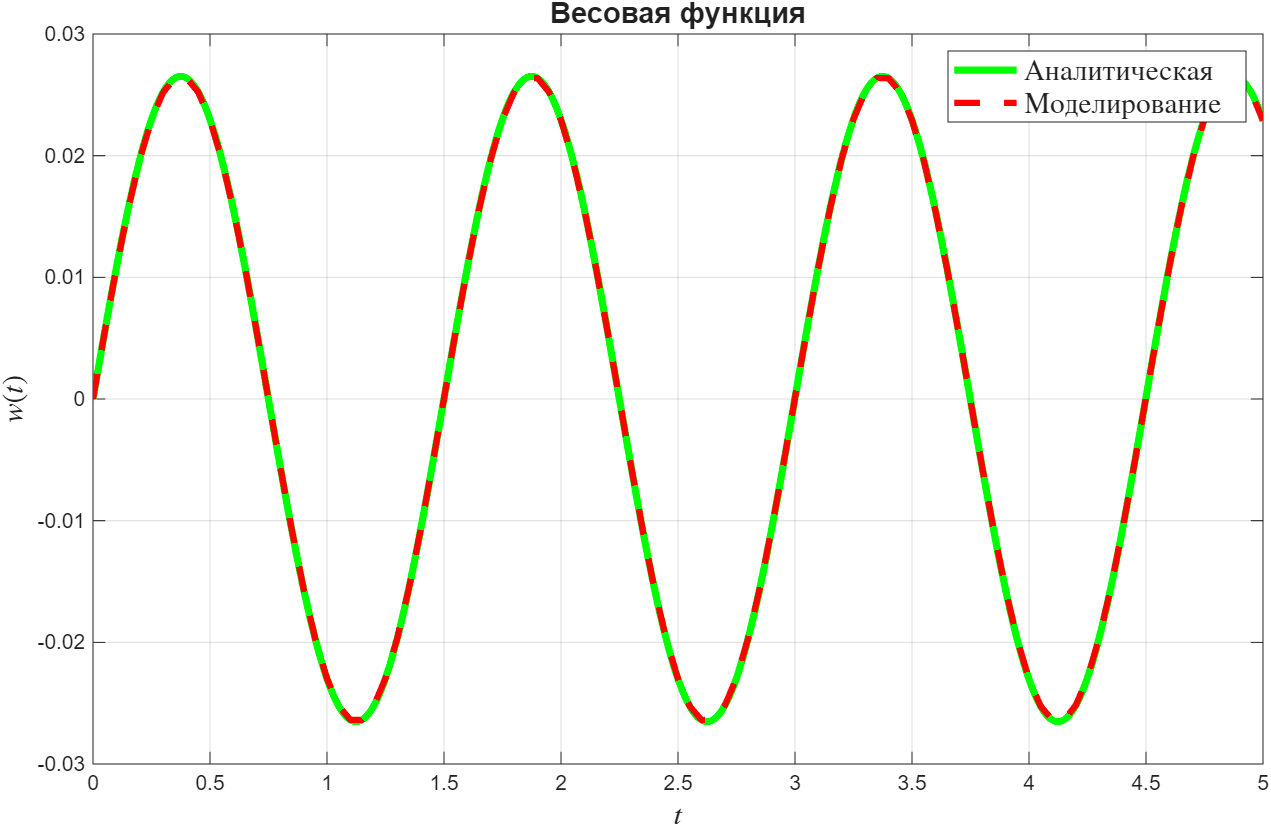
\includegraphics[width=0.84\linewidth]{images/Figure_5_4_1.png}
    \caption{График сравнения весовых характеристик}
    \label{fig:placeholder}
\end{figure}

\begin{figure}[H]
    \centering
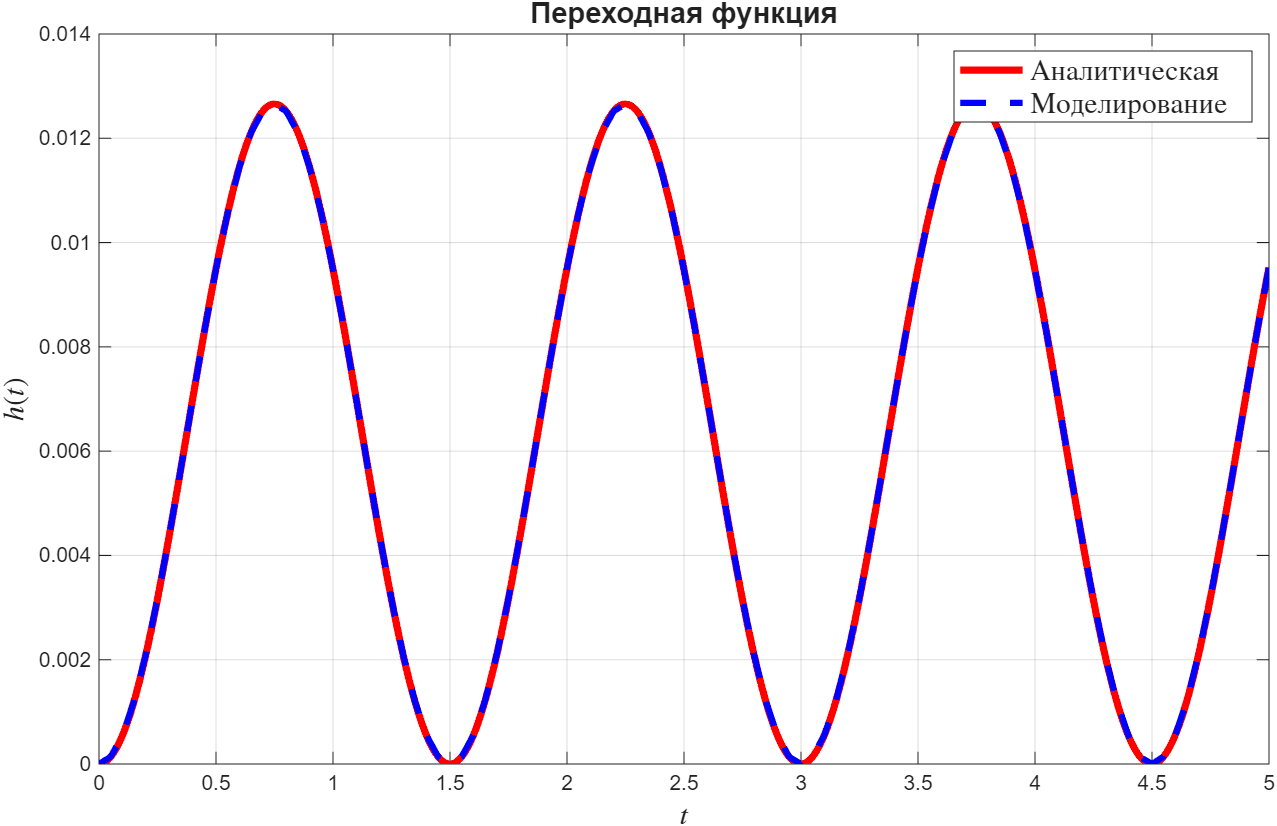
\includegraphics[width=0.84\linewidth]{images/Figure_5_4_2.png}
    \caption{График сравнения переходных характеристик}
    \label{fig:placeholder}
\end{figure}

\begin{figure}[H]
    \centering
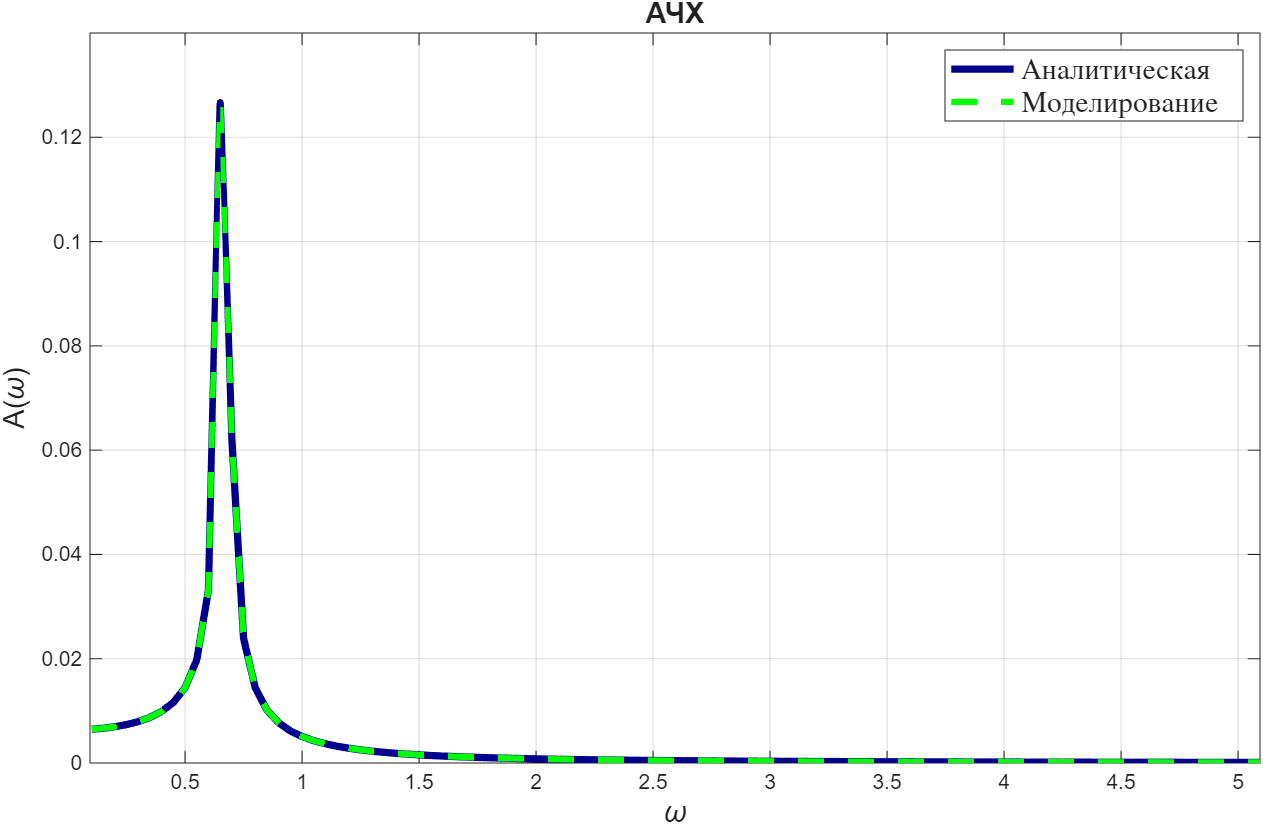
\includegraphics[width=0.84\linewidth]{images/Figure_5_4_3.png}
    \caption{График сравнения АЧХ}
    \label{fig:placeholder}
\end{figure}

\begin{figure}[H]
    \centering
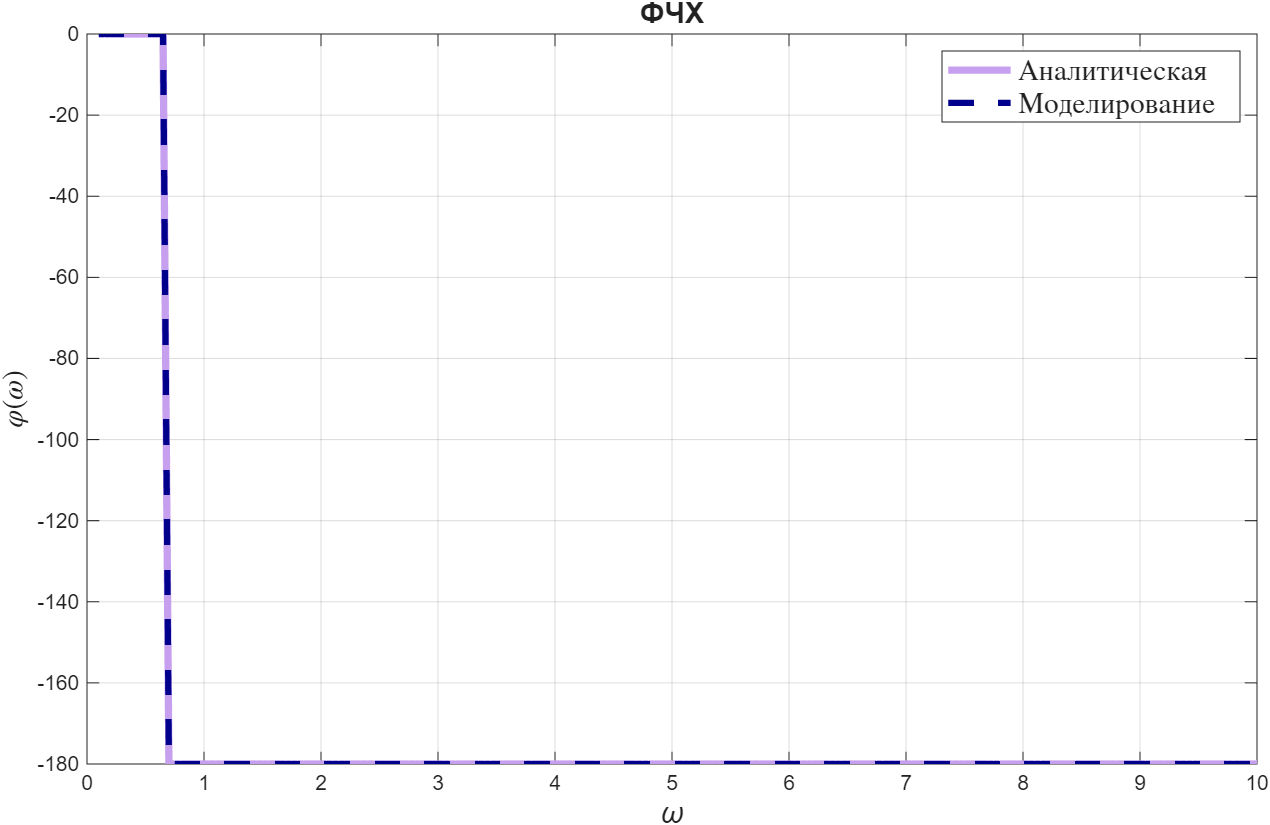
\includegraphics[width=0.84\linewidth]{images/Figure_5_4_4.png}
    \caption{График сравнения ФЧХ}
    \label{fig:placeholder}
\end{figure}

\begin{figure}[H]
    \centering
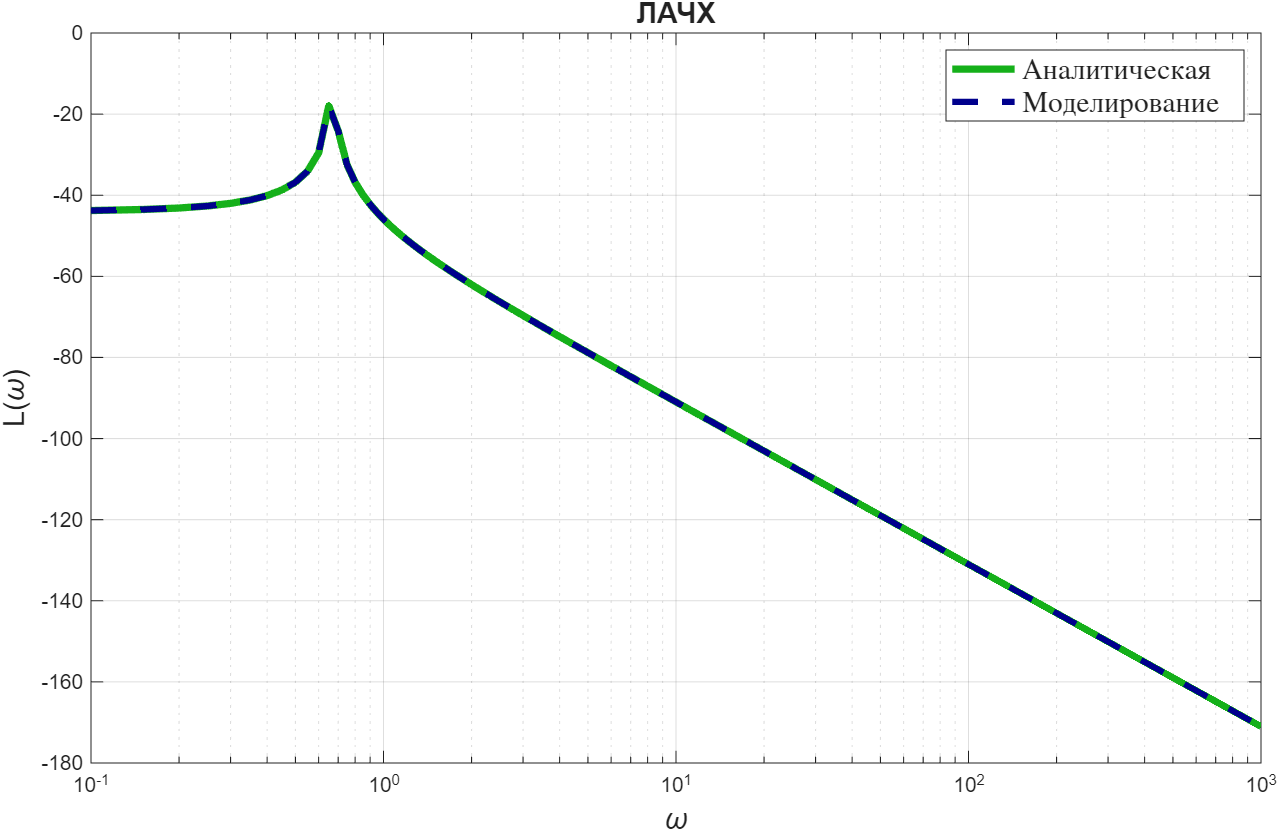
\includegraphics[width=0.84\linewidth]{images/Figure_5_4_5.png}
    \caption{График сравнения ЛАЧХ}
    \label{fig:placeholder}
\end{figure}

\begin{figure}[H]5
    \centering
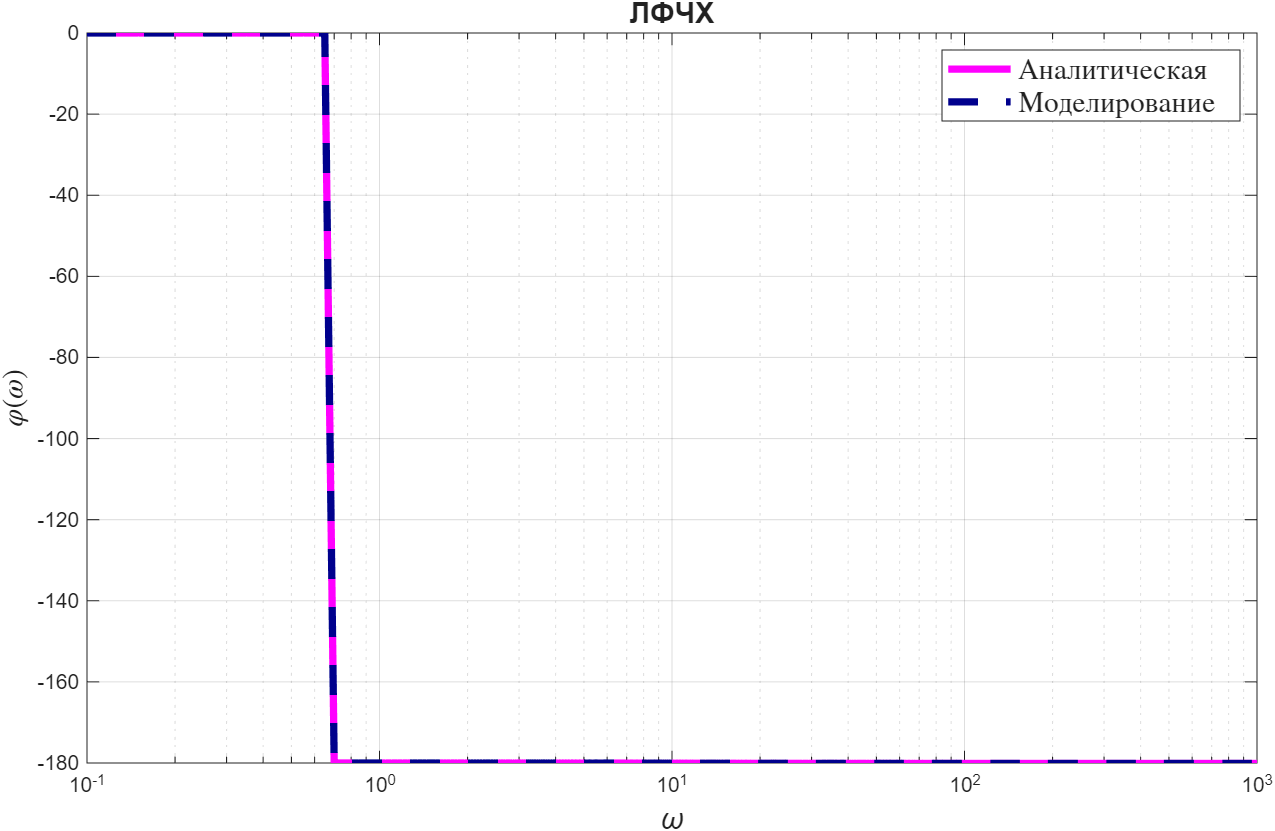
\includegraphics[width=0.84\linewidth]{images/Figure_5_4_6.png}
    \caption{График сравнения ЛФЧХ}
    \label{fig:placeholder}
\end{figure}

Как можно заметить, что графики полностью совпадают, на предложенных промежутках, что даёт понять, что все проделанные вычисления верны.

\subsection{Выводы}

Система является консервативным звеном, что подтверждается незатухающими колебаниями на графиках переходной и весовой функций. 




\section{Объект 5. Что ты такое?}

\subsection{Исходные данные}
\begin{center}
\begin{tabular}{|c|c|}
\hline
Параметр & Значение \\
\hline
$R_1$ & 5542 \,Ом \\
\hline
$R_2$ & 15975 \,Ом \\
\hline
$C$ & 388\, мкФ  \\
\hline
\end{tabular}
\end{center}

\begin{figure}[H]
    \centering
    \includegraphics[width=0.75\linewidth]{images/image_5_2.png}
    \caption{Принципиальная схема регулятора на операционном усилителе}
    \label{fig:placeholder}
\end{figure}

Входом объекта считаем $U_{\text{вх}}(t)$, а выходом $U_{\text{вых}}(t)$.

\subsection{Вывод передаточной функции}

Исходя из информации из дополнительных источников делаем вывод, что перед нами ПИ-регулятор

\[
W(s) =\dfrac{R_2}{R_1}+\frac{1}{CR_1s}
\]

\[
K = \frac{R_2}{R_1}, \quad T = CR_1 
\]

\[
W(s) = \frac{1}{Ts} + K = \frac{KTs + 1}{Ts}
\]
\textbf{тип звена:} изодромное звено
\subsection{Аналитические выражения временны́х характеристик}

\textbf{Весовая характеристика} $w(t)$:
\[
w(t) = \mathcal{L}^{-1}\{W(s)\}
\]
\[
w(t) =\mathcal{L}^{-1}\{W(s)\}= \mathcal{L}^{-1}\left\{\frac{1}{Ts} + K\right\} =\frac{1}{T} + K \cdot \delta(t)
\]

\vspace{5mm}
\textbf{Переходная характеристика} $h(t)$:
\[
h(t) = \mathcal{L}^{-1}\left\{W(s) \cdot \frac{1}{s}\right\} = \mathcal{L}^{-1}\left\{\left(\frac{1}{Ts} + K\right) \cdot \frac{1}{s}\right\} = \frac{1}{T}t + K \cdot 1(t)
\]


\subsection{Аналитические выражения частотных характеристик}
Частотная передаточная функция:
\[
W(j\omega) = K+ \frac{1}{T(j\omega)} = K - \frac{j}{T\omega}
\]

Выделим действительную $P(\omega)$ и мнимую $Q(\omega)$ части:
\[
P(\omega) = K, \quad Q(\omega) = -\frac{1}{T\omega}
\]

\textbf{Амплитудно-частотная характеристика:}
\[
A(\omega) = \sqrt{P(\omega)^2 + Q(\omega)^2} = \sqrt{K^2 + \left( -\frac{1}{T\omega} \right)^2} = \sqrt{K^2 + \frac{1}{(T\omega)^2}}
\]

\textbf{Фазо-частотная характеристика:}
\[
\varphi(\omega) = \operatorname{atan2}(Q(\omega), P(\omega)) = \operatorname{atan2}\left( -\frac{1}{T\omega}, K \right)
\]

\[
\varphi(\omega) = -\arctan\left(\frac{1}{KT\omega}\right)
\]

\textbf{Логарифмическая амплитудно-частотная характеристика:}
\[
L(\omega) = 20 \lg(A(\omega)) = 20 \lg \left( \sqrt{K^2 + \frac{1}{(T\omega)^2}} \right)
\]

\subsection{Моделирование в MATLAB}

\begin{figure}[H]
    \centering
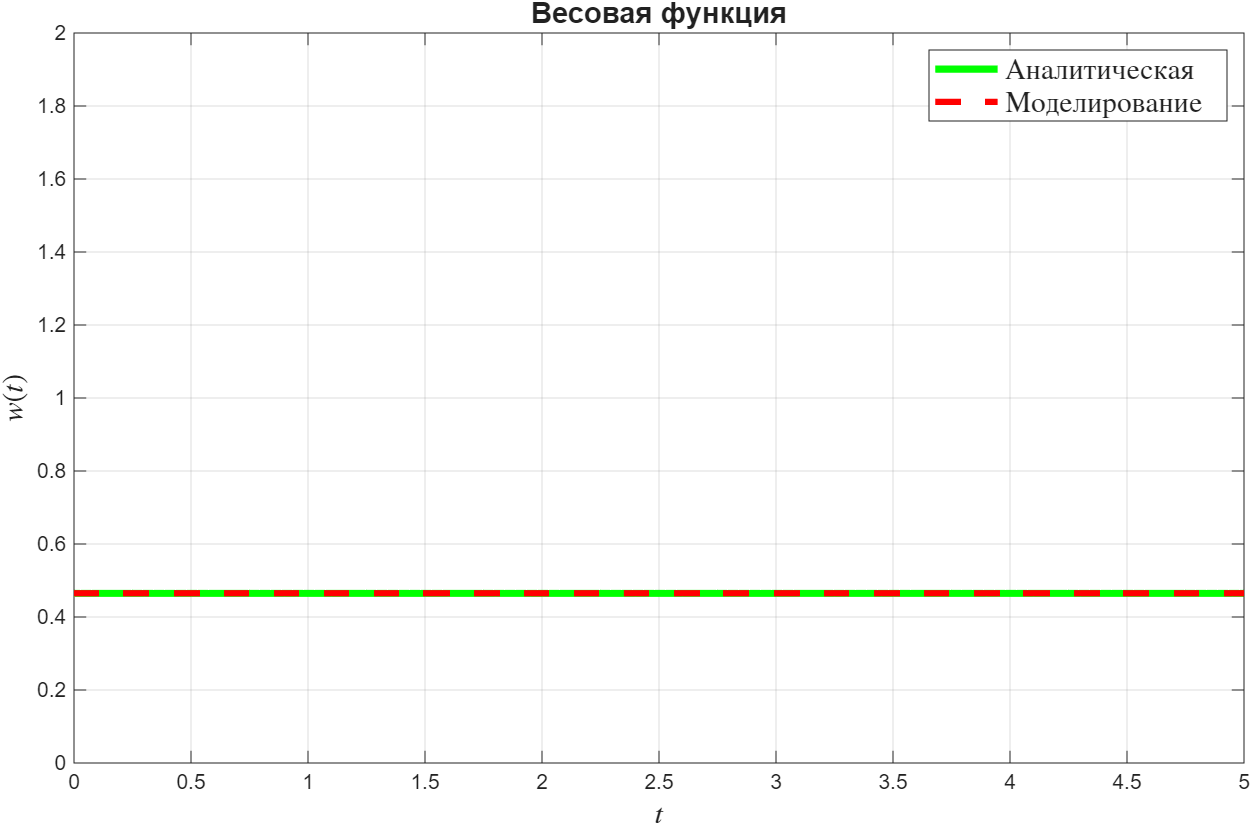
\includegraphics[width=0.84\linewidth]{images/Figure_5_5_1.png}
    \caption{График сравнения весовых характеристик}
    \label{fig:placeholder}
\end{figure}

\begin{figure}[H]
    \centering
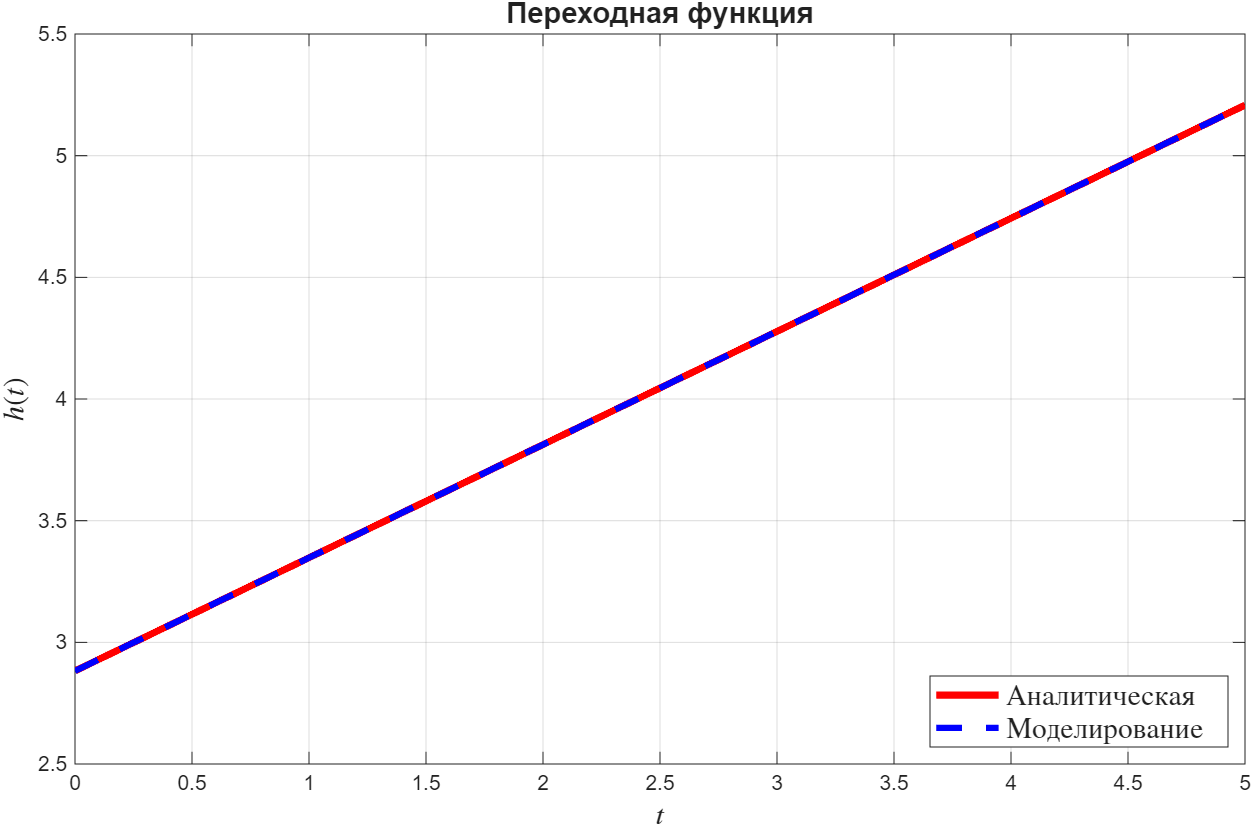
\includegraphics[width=0.84\linewidth]{images/Figure_5_5_2.png}
    \caption{График сравнения переходных характеристик}
    \label{fig:placeholder}
\end{figure}

\begin{figure}[H]
    \centering
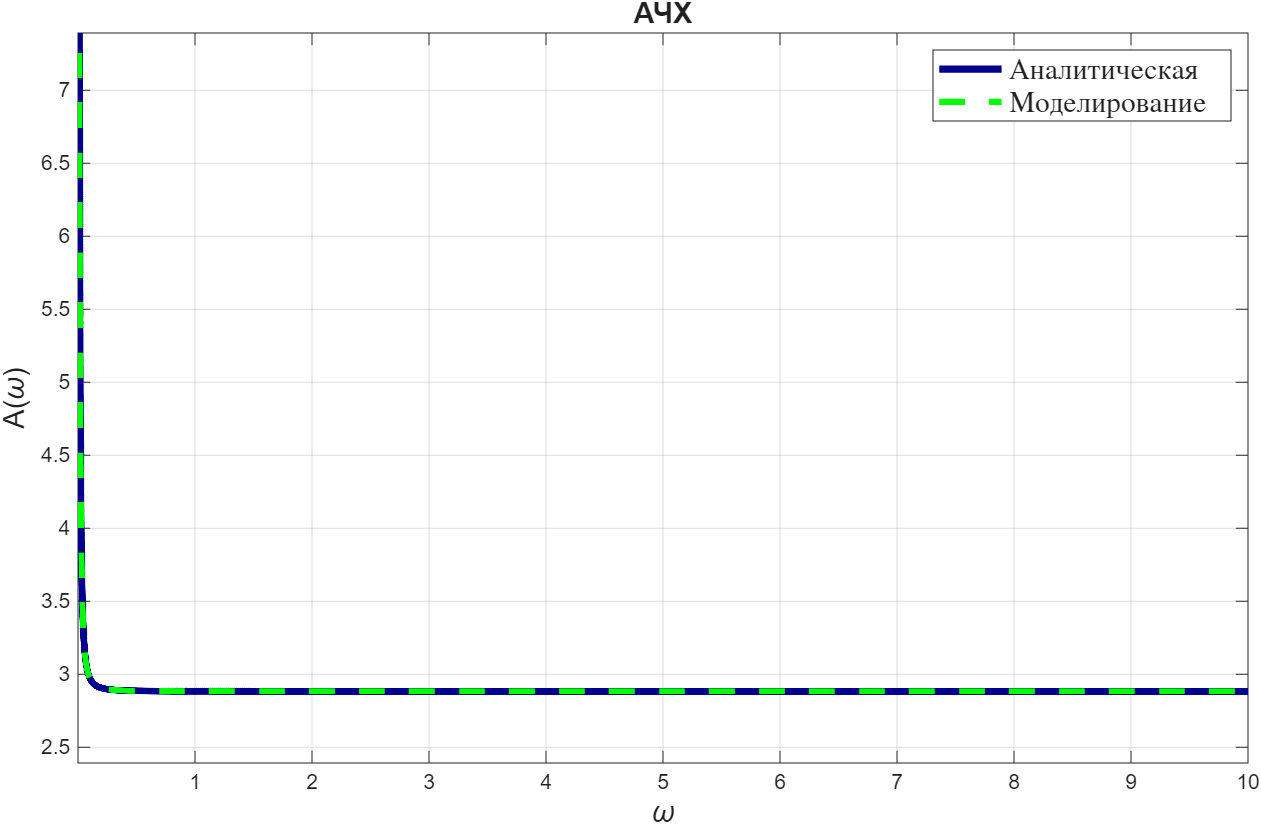
\includegraphics[width=0.84\linewidth]{images/Figure_5_5_3.png}
    \caption{График сравнения АЧХ}
    \label{fig:placeholder}
\end{figure}

\begin{figure}[H]
    \centering
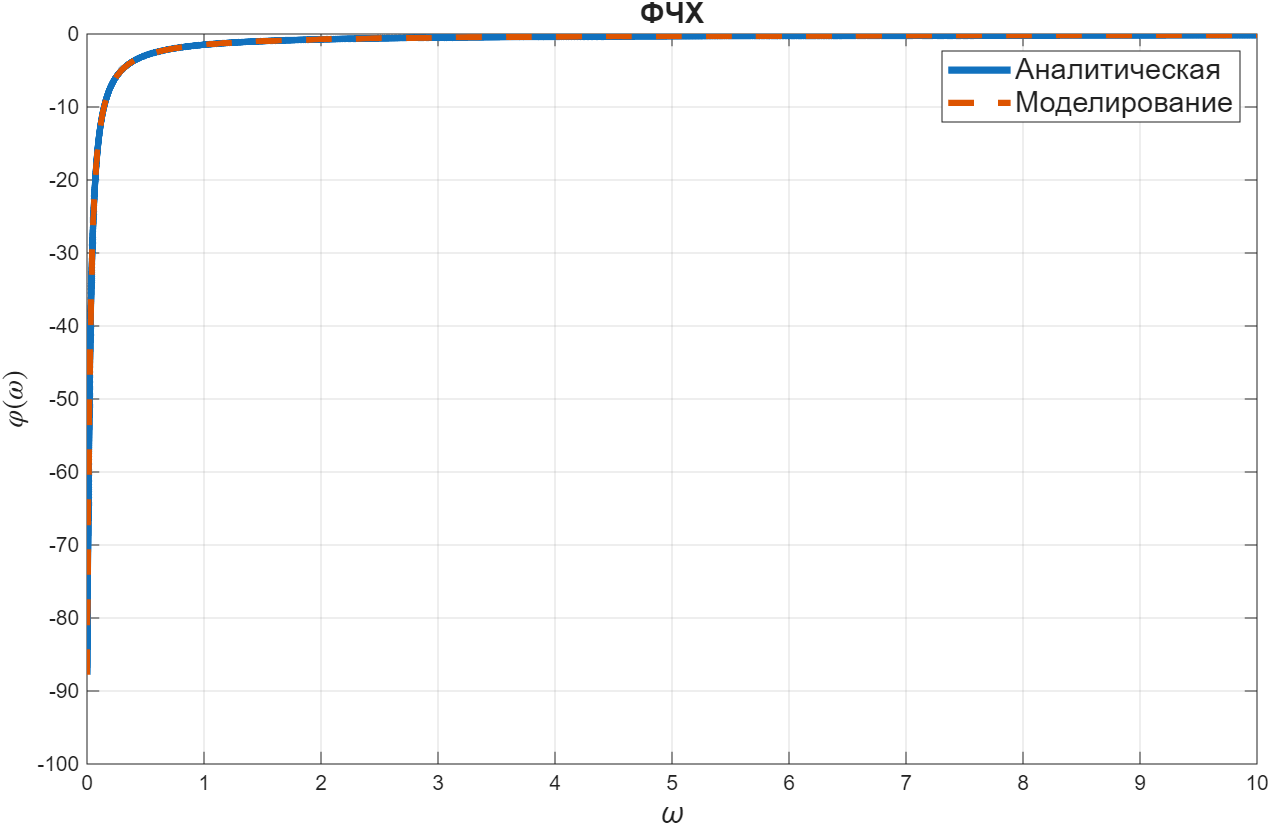
\includegraphics[width=0.84\linewidth]{images/Figure_5_5_4.png}
    \caption{График сравнения ФЧХ}
    \label{fig:placeholder}
\end{figure}

\begin{figure}[H]
    \centering
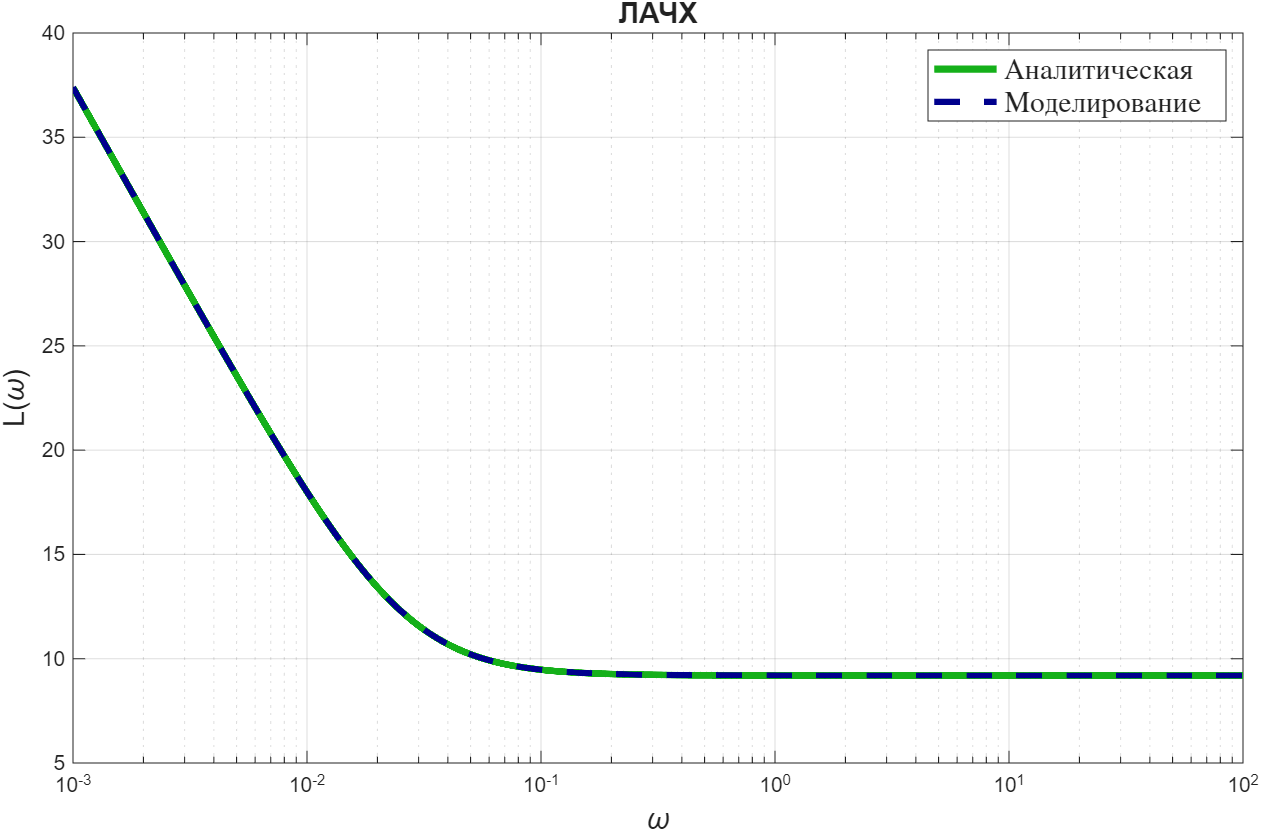
\includegraphics[width=0.84\linewidth]{images/Figure_5_5_5.png}
    \caption{График сравнения ЛАЧХ}
    \label{fig:placeholder}
\end{figure}

\begin{figure}[H]
    \centering
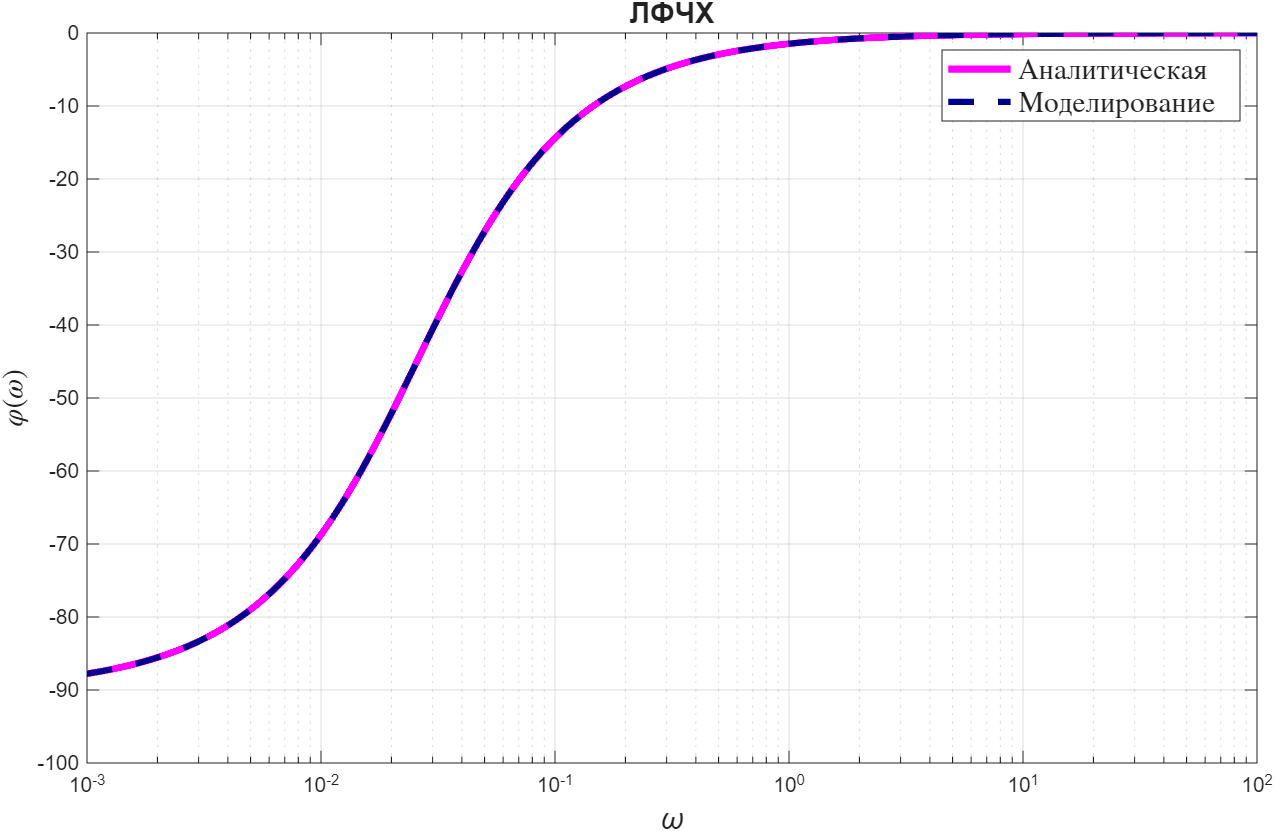
\includegraphics[width=0.84\linewidth]{images/Figure_5_5_6.png}
    \caption{График сравнения ЛФЧХ}
    \label{fig:placeholder}
\end{figure}

Как можно заметить, что графики полностью совпадают, на предложенных промежутках, что даёт понять, что все проделанные вычисления верны.

\subsection{Выводы}
Схема является реальным дифференцирующим звеном. Схема выполняет функцию пропорционально-интегрального регулятора.





\section{Вывод}

В ходе лабораторной работы было выполнено исследование пяти динамических систем с целью их идентификации как стандартных динамических звеньев. \\
Каждый объект успешно описан стандартной передаточной функцией.\\
Результаты компьютерного моделирования в полностью совпали с аналитически рассчитанными временными и частотными характеристиками, что верифицирует корректность построенных математических моделей и выполненных преобразований.

\section{Приложение}

\begin{lstlisting}[language=Matlab]
k_m = 0.3611;
k_e = 0.3611;
R = 4.6775;
J = 0.0024;

K = 1/k_e;
T = (J * R) / (k_m * k_e);
W = tf(K, [T 1]);

t = 0:0.01:5;

w_analytical = (K/T) * exp(-t/T);

h_analytical = K * (1 - exp(-t/T));

[w_sim, t_w] = impulse(W, 5);

[h_sim, t_h] = step(W, 5);

h = figure;
plot(t, w_analytical, 'g', 'LineWidth', 2);
hold on;
plot(t_w, w_sim, 'r', 'LineStyle', '-.', 'LineWidth', 1.5);
grid on;
title('Весовая функция', 'FontSize', 14);
xlabel('$$t$$', 'Interpreter','latex');
ylabel('$$f(t)$$', 'Interpreter','latex');
xlim([0, 1]);
legend('Аналитическая','моделирование','Interpreter','latex', 'Location','northeast');
exportgraphics(h,'w_1.png','Resolution', 600);

h1 = figure;
plot(t, h_analytical, 'r', 'LineWidth', 2);
hold on;
plot(t_h, h_sim, 'b', 'LineStyle', '-.', 'LineWidth', 1.5);
grid on;
title('Переходная функция', 'FontSize', 14);
xlabel('$$t$$', 'Interpreter','latex');
ylabel('$$f(t)$$', 'Interpreter','latex');
xlim([0, 1]);
legend('Аналитическая','моделирование','Interpreter','latex', 'Location','southeast');
exportgraphics(h1,'h_1.png','Resolution', 600);

freqs = linspace(0.1, 1000, 20000);
omega = 2*pi*freqs;
[mag, phase, ~] = bode(W, omega);
mag_analytical = k_m ./ (sqrt(k_m^2 * k_e^2 + (J * R .* omega).^2));
phase_analytical = atan(-omega .* T) .* 180 ./ pi;
mag = squeeze(mag);
phase = squeeze(phase);
h = figure;
plot(freqs, mag_analytical, 'Color', '#00008d', 'LineWidth', 1.5);
grid on;
hold on;
plot(freqs, mag, 'g', 'LineWidth', 1, 'LineStyle', '--');
title('АЧХ');
xlabel('\omega');
ylabel('A(\omega)');
legend('$A(\omega)$','Interpreter','latex', 'Location','northeast');
xlim([0, 200]);
legend('Аналитическая','моделирование','Interpreter','latex', 'Location','northeast');
exportgraphics(h,'ach_1.png','Resolution', 600);

h1 = figure;
plot(freqs, phase_analytical, 'Color', '#c79fef', 'LineWidth', 1.5);
grid on;
hold on;
plot(freqs, phase, 'Color', '#00008d', 'LineWidth', 1, 'LineStyle', '-.');
title('ФЧХ');
xlabel('\omega');
ylabel('$$\varphi(\omega)$$', 'Interpreter','latex');
xlim([0, 200]);
legend('Аналитическая','моделирование','Interpreter','latex', 'Location','northeast');
exportgraphics(h1,'fch_1.png','Resolution', 600);
mag_dB = 20*log10(mag);
mag_dB_analytic = 20*log10(mag_analytical);

h2 = figure;
semilogx(freqs, mag_dB_analytic, 'Color', '#15b01a', 'LineWidth', 1.5);
grid on;
hold on;
semilogx(freqs, mag_dB, 'Color', '#00008d', 'LineWidth', 1, 'LineStyle', '--');
title('ЛАЧХ');
xlabel('\omega');
ylabel('L(\omega)');
legend('Аналитическая','моделирование','Interpreter','latex', 'Location','northeast');
exportgraphics(h2,'lach_1.png','Resolution', 600);

h3 = figure;
semilogx(freqs, phase_analytical, 'Color', '#ff00ff', 'LineWidth', 1.5, 'LineStyle', '--');
grid on;
hold on;
semilogx(freqs, phase, 'Color', '#00008d', 'LineWidth', 1.5, 'LineStyle', ':');
title('ЛФЧХ');
xlabel('\omega');
ylabel('$$\varphi(\omega)$$', 'Interpreter','latex');
legend('ЛФЧХ', '0°', '-90°', 'Location', 'best');
legend('Аналитическая','моделирование','Interpreter','latex', 'Location','northeast');
exportgraphics(h3,'lfch_1.png','Resolution', 600);
\end{lstlisting}
\end{document}